%%%%%%%%%%%%%%%%%%%%%%%%%%%%%%%%%%%%%%%%%%%%%%%%%%%%%%%%%%%%%%%%%%%%%%
% Overleaf (WriteLaTeX) Example: Molecular Chemistry Presentation
%
% Source: http://www.overleaf.com
%
% In these slides we show how Overleaf can be used with standard
% chemistry packages to easily create professional presentations.
%
% Feel free to distribute this example, but please keep the referral
% to overleaf.com
%
%%%%%%%%%%%%%%%%%%%%%%%%%%%%%%%%%%%%%%%%%%%%%%%%%%%%%%%%%%%%%%%%%%%%%%

\documentclass[xcolor={dvipsnames}]{beamer}

\mode<presentation>
{
  \usetheme{Madrid}       % or try default, Darmstadt, Warsaw, ...
  \usecolortheme{default} % or try albatross, beaver, crane, ...
  \usefonttheme{default}    % or try default, structurebold, ...
  \setbeamertemplate{navigation symbols}{}
  \setbeamertemplate{caption}[numbered]
}

\usepackage[english]{babel}
\usepackage[utf8x]{inputenc}
\usepackage{graphicx}
\usepackage{hyperref}
  \hypersetup{colorlinks=true}
  \hypersetup{urlcolor=blue}
  \hypersetup{linkcolor = .}
\usepackage{xcolor}
\usepackage{siunitx}
  \sisetup{separate-uncertainty = true}
\DeclareSIUnit\barn{b}
\usepackage{physics}
\usepackage[font=small,labelfont=bf]{caption}
\usepackage{subcaption}
\usepackage[en-GB]{datetime2}
\usepackage{overpic}
\usepackage{feynmp}
\DeclareGraphicsRule{*}{mps}{*}{}
\usepackage{scalerel}
\newcommand{\mylbrace}[2]{\vspace{#2pt}\hspace{6pt}\scaleleftright[\dimexpr5pt+#1\dimexpr0.06pt]{\lbrace}{\rule[\dimexpr2pt-#1\dimexpr0.5pt]{-4pt}{#1pt}}{.}}
\newcommand{\myrbrace}[2]{\vspace{#2pt}\scaleleftright[\dimexpr5pt+#1\dimexpr0.06pt]{.}{\rule[\dimexpr2pt-#1\dimexpr0.5pt]{-4pt}{#1pt}}{\rbrace}\hspace{6pt}}

% Trim in percent
\usepackage{adjustbox}

% No "Figure" prefix
\setbeamertemplate{caption}{\raggedright\insertcaption\par}

% Nice decay amplitude diagrams
\usepackage{amsmath,amssymb,tikz-cd}

% Strike out text
\usepackage[normalem]{ulem}

% For figures with text overlay
\usepackage{overpic}

% Arrows
\usepackage{tikz}
\newcommand{\tikzmark}[1]{\tikz[remember picture] \node[coordinate] (#1) {#1};}

% Colourbox with line breaks
\newcommand{\cbox}[2][lime!20]{%
  \colorbox{#1}{\parbox{\dimexpr\linewidth-2\fboxsep}{\strut #2\strut}}%
}

% Vector arrows
\usepackage[pdftex]{pict2e}

% Checkmark symbol
\def\checkmark{\tikz\fill[scale=0.4](0,.35) -- (.25,0) -- (1,.7) -- (.25,.15) -- cycle;}

% Copy code
\usepackage{listings}
\lstset{
  basicstyle=\ttfamily\tiny,
  breaklines=true
}

% Here's where the presentation starts, with the info for the title slide
\title[A\&S week]{Tracking efficiencies from \texorpdfstring{$J/\psi\to\mu^+\mu^-$}{JpsiToMuMu}}

\author[Martin Tat]{Rowina Caspary$^1$, Michel De Cian$^2$, Fabian Glaser$^1$, Stephanie Hansmann-Menzemer$^1$, Peilian Li$^3$, Maurice Morgenthaler$^1$, \\ \textbf{Martin Tat}$^1$}
\institute[Heidelberg]{Heidelberg University$^1$, University of Manchester$^2$, UCAS$^3$}
\date{5th March 2026}

\titlegraphic{
\includegraphics[height = 1.2cm]{../lhcb.jpg}\hspace{1.0cm}~%
              
\includegraphics[height = 1.2cm]{../FSP_logo.png}
              
\includegraphics[height = 1.2cm]{../ManchesterLogo.jpg}~%
              
\includegraphics[height = 1.2cm]{../UCAS_logo.png}~%
              
\includegraphics[height = 1.2cm]{../HeidelbergLogo.pdf}}

\begin{document}

\begin{frame}
  \titlepage
\end{frame}

% These three lines create an automatically generated table of contents.
%\begin{frame}{Outline}
%  \tableofcontents
%\end{frame}

\begin{frame}{Introduction}
  \vspace{0.0cm}
  {\Large Strategy for tracking efficiency determination:}
  \vspace{0.2cm}
  \begin{itemize}
    \setlength\itemsep{0.8em}
    \item{Tag-and-probe method with $J/\psi\to\mu^+\mu^-$}
    \item{Combine efficiencies of two methods:}
    \begin{itemize}
      \item{VeloMuon: SciFi efficiency}
      \item{Downstream: Velo efficiency}
      \item{Combined: Velo $\times$ SciFi efficiencies}
    \end{itemize}
    \item{Cross check with long track efficiency with the MuonUT method}
    \begin{itemize}
      \item{Main systematic}
    \end{itemize}
  \end{itemize}
\end{frame}

\begin{frame}{Tag-and-probe method}
  \vspace{0.0cm}
  \begin{figure}[htb]
    \centering
    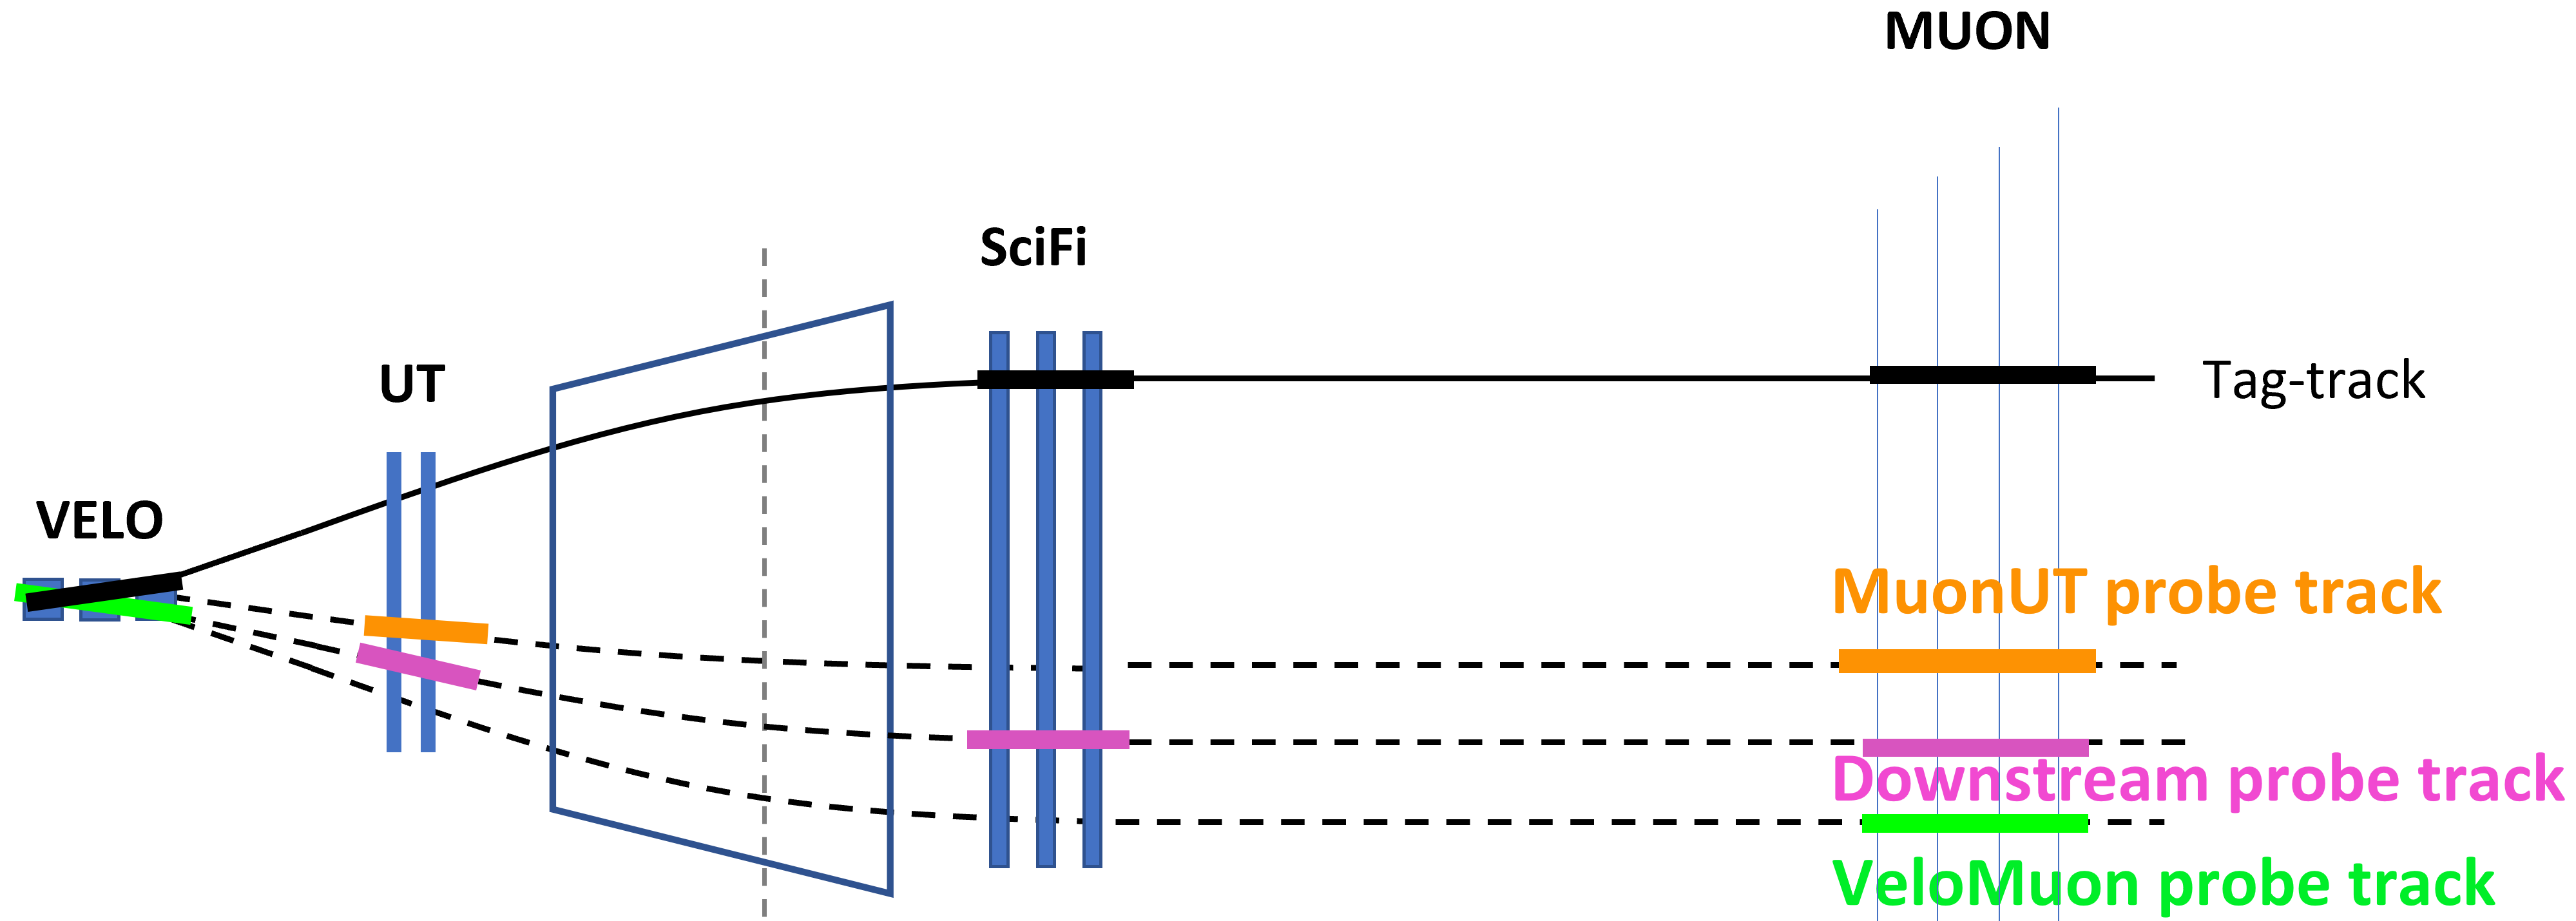
\includegraphics[width=0.75\textwidth]{Plots/Tag_and_probe_method.png}
    \caption*{\small Figure by Rowina}
  \end{figure}
  \begin{itemize}
    \item{Fully reconstruct one muon from $J/\psi\to\mu^+\mu^-$}
    \item{Partially reconstruct the other muon}
    \item{Match hits in specific sub-detector with partially reconstructed track}
  \end{itemize}
  \begin{equation*}
    \epsilon_{\rm track} = \frac{N_{\rm matched}}{N_{\rm matched} + N_{\rm failed}}
  \end{equation*}
\end{frame}

\begin{frame}{Overlap criteria in matching}
  \vspace{0.0cm}
  {Matching is done by comparing the hits of the probe track with a long track in each subdetector}
  \vspace{0.2cm}
  \begin{center}
    \begin{tabular}{ccccc}
      \hline
      Method     & Velo     & UT              & SciFi    & Muon \\
      \hline
      VeloMuon   & $> 40\%$ & --              & --       & $> 40\%$ \\
      Downstream & --       & --              & $> 40\%$ & $> 40\%$ \\
      MuonUT     & --       & $0$ or $> 40\%$ & --       & $> 40\%$ \\
      \hline
    \end{tabular}
  \end{center}
  {Note:}
  \begin{itemize}
    \item{Matching was originally performed in a trigger line}
    \item{We now have functors for direct access to overlap fractions}
    \item{Requires rerunning reconstruction in 2024, as long-track information was not persisted}
  \end{itemize}
\end{frame}

\begin{frame}{Motivation and strategy}
  \vspace{0.0cm}
  {\Large Why do we care?}
  \vspace{0.2cm}
  \begin{itemize}
    \setlength\itemsep{0.8em}
    \item{Imperfect modelling of track reconstruction efficiency in MC}
    \item{Physics analyses that rely on efficiencies from MC must correct for this by reweighting}
  \end{itemize}
  \vspace{0.3cm}
  {\Large What do we provide?}
  \vspace{0.2cm}
  \begin{enumerate}
    \item{Tracking efficiency ratio between data/MC of muon long tracks}
    \begin{itemize}
      \setlength\itemsep{0.2em}
      \item{Long track efficiency from product of Velo and SciFi efficiencies}
      \item{2D $p$--$\eta$ binning}
      \item{Dominant systematic uncertainty from MuonUT-Combined difference}
    \end{itemize}
    \item{Hadronic corrections for pions, kaons and protons}
    \begin{itemize}
      \setlength\itemsep{0.2em}
      \item{Mainly due to uncertainty in material budget}
      \item{Using binning in $\eta$, with the same bin edges as for muons}
    \end{itemize}
  \end{enumerate}
\end{frame}

\begin{frame}{Overview of previous work}
  \vspace{0.0cm}
  {Long history of previous work}
  \vspace{0.2cm}
  \begin{itemize}
    \setlength\itemsep{1.0em}
    \item{Method and results carefully documented in Rowina's thesis \href{https://repository.cern/records/n2g9v-81z15}{here}}
    \item{Latest presentations in RTA-WP4 on}
    \begin{itemize}
      \item[-]{muon tracking efficiencies \href{https://indico.cern.ch/event/1577595/\#4-update-track-reconstruction}{here}}
      \item[-]{hadronic corrections \href{https://indico.cern.ch/event/1577599/\#3-hadronic-tracking-uncertaint}{here}}
    \end{itemize}
  \end{itemize}
  \vspace{0.5cm}
  {Tracking efficiencies are determined using TrackCalib2}
  \vspace{0.2cm}
  \begin{itemize}
    \setlength\itemsep{0.8em}
    \item{GitLab repository \href{https://gitlab.cern.ch/lhcb-rta/trackcalib2}{here}}
    \item{Mass fit done on tuples from AP to extract efficiencies}
    \item{Note: Analysts should \underline{not} have to run TrackCalib2 themselves, unless the released numbers are not suitable (need different binning, etc)}
  \end{itemize}
\end{frame}

\begin{frame}{Datasets considered}
  \vspace{0.0cm}
  {\large Datasets considered:}
  \vspace{0.2cm}
  \begin{itemize}
    \setlength\itemsep{1.0em}
    \item{2024}
    \begin{itemize}
      \item[-]{Analysis of blocks 2, 1, 5, 6, 7, 8, $pp$ ref mostly done}
      \item[-]{Currently waiting for large MC production to finish}
      \item[-]{Blocks 4 and 3 don't have MC yet}
    \end{itemize}
    \item{2025}
    \begin{itemize}
      \item[-]{Analysis in progress}
      \item[-]{Will request 2025 post-TS MC soon}
    \end{itemize}
    \item{2026}
    \begin{itemize}
      \item[-]{Plan to look at soon}
    \end{itemize}
  \end{itemize}
\end{frame}

\begin{frame}{Remarks on current results}
  \vspace{0.0cm}
  {\large Remark on phase-space differences between 2024 and 2025:}
  \vspace{0.2cm}
  \begin{itemize}
    \setlength\itemsep{1.0em}
    \item{Probe muon $p_T$ cut was at $500$~MeV in 2024}
    \item{Loosened to $100$~MeV in 2025}
    \item{Therefore cannot compare 2024 and 2025 directly}
  \end{itemize}
\end{frame}

\begin{frame}{Example mass fit}
  \vspace{0.0cm}
  {\large Example of mass fit to extract tracking efficiency}
  \begin{figure}[htb]
    \centering
    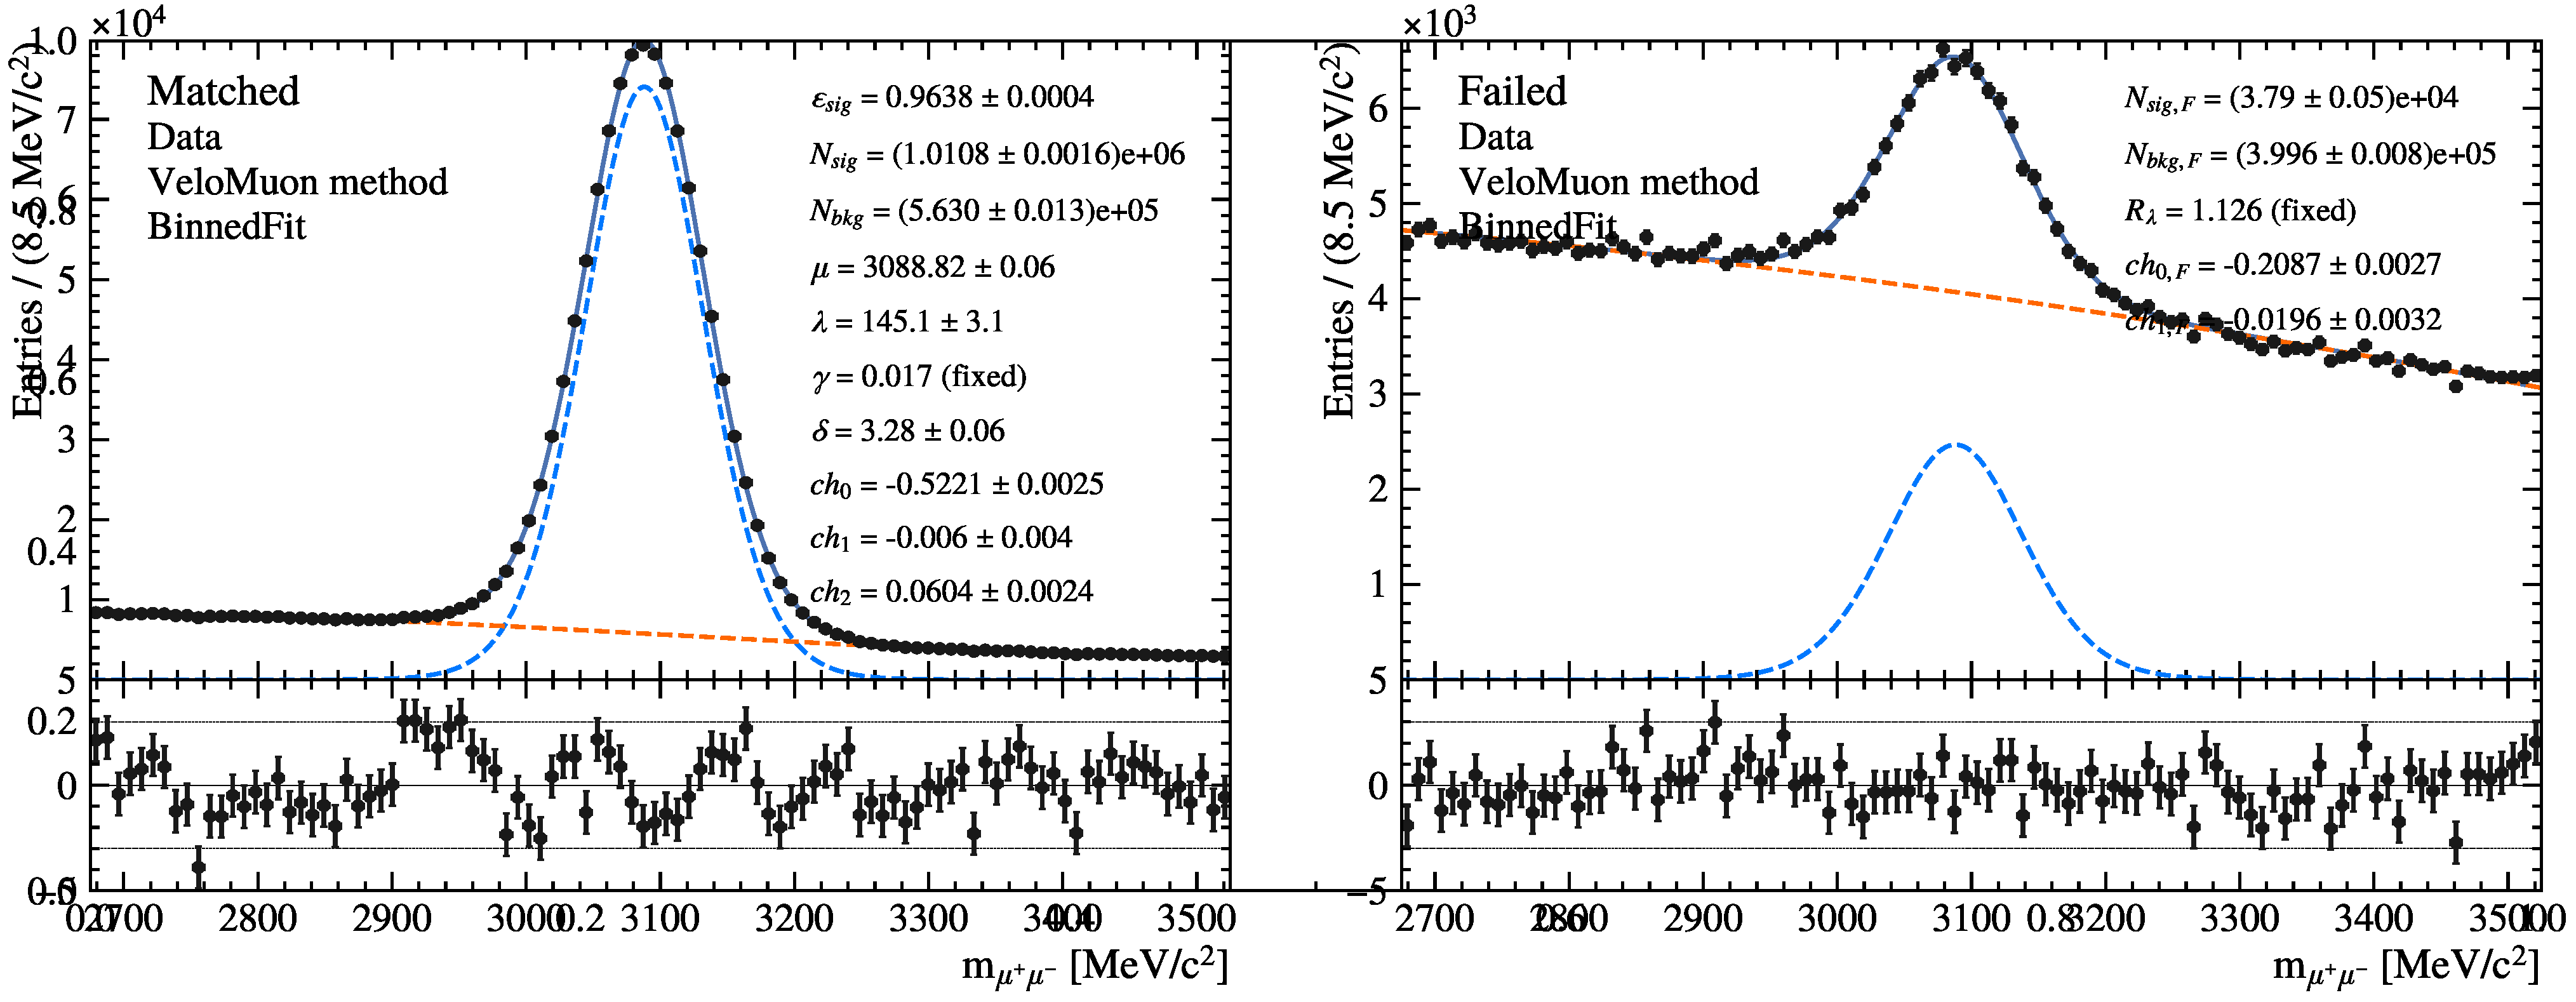
\includegraphics[width=0.85\textwidth]{Plots/Data_VeloMuon_ETA_3_sim.pdf}
  \end{figure}
  \begin{itemize}
    \item{Efficiency is a free parameter in the fit}
    \item{Matched and failed samples simultaneously fitted to ensure correct uncertainties}
  \end{itemize}
\end{frame}

\begin{frame}{Efficiency comparisons}
  \vspace{0.0cm}
  {\large Comparison of SciFi tracking efficiencies in all data blocks}
  \begin{figure}[htb]
    \centering
    \begin{subfigure}{0.5\textwidth}
      \centering
      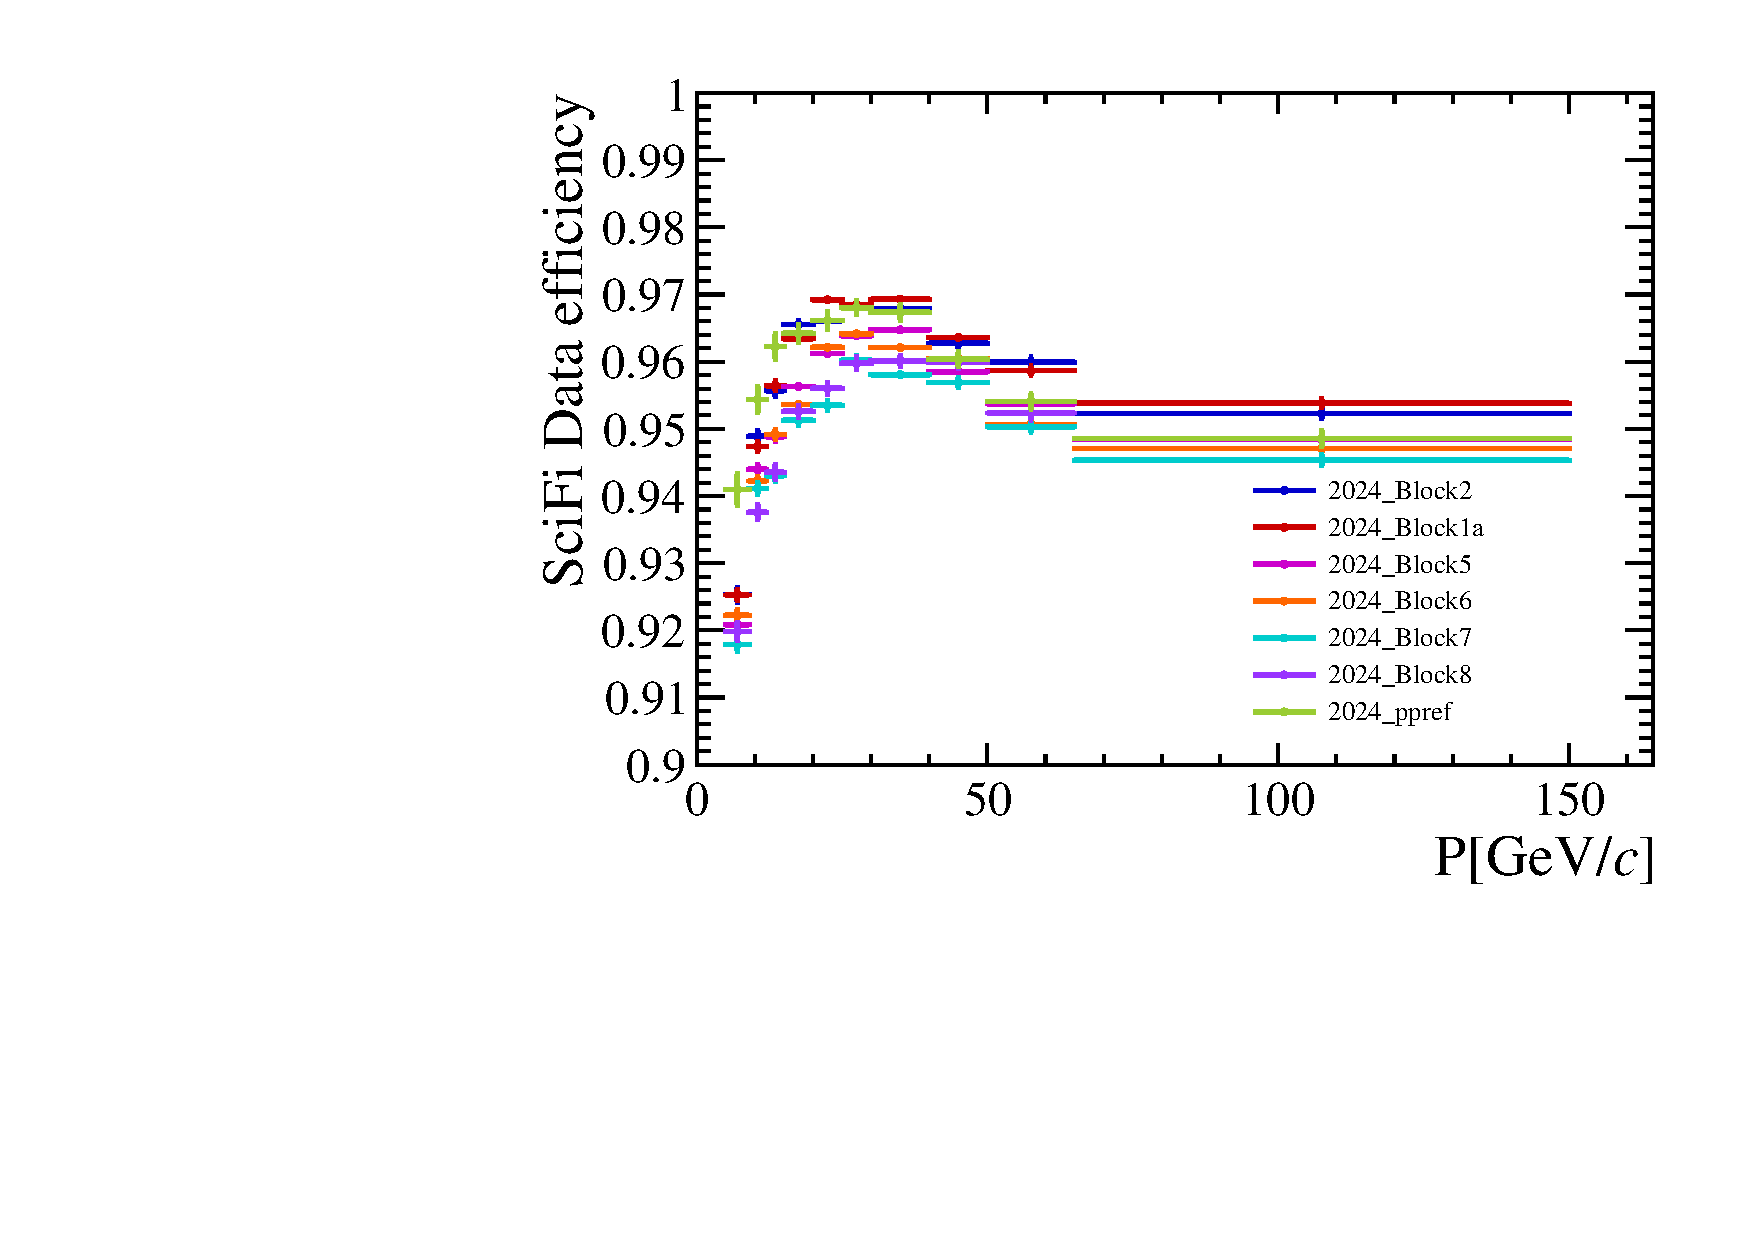
\includegraphics[width=0.75\textwidth]{Plots/trackeff_Data_VeloMuon_P_respruced_samples.pdf}
    \end{subfigure}%
    \begin{subfigure}{0.5\textwidth}
      \centering
      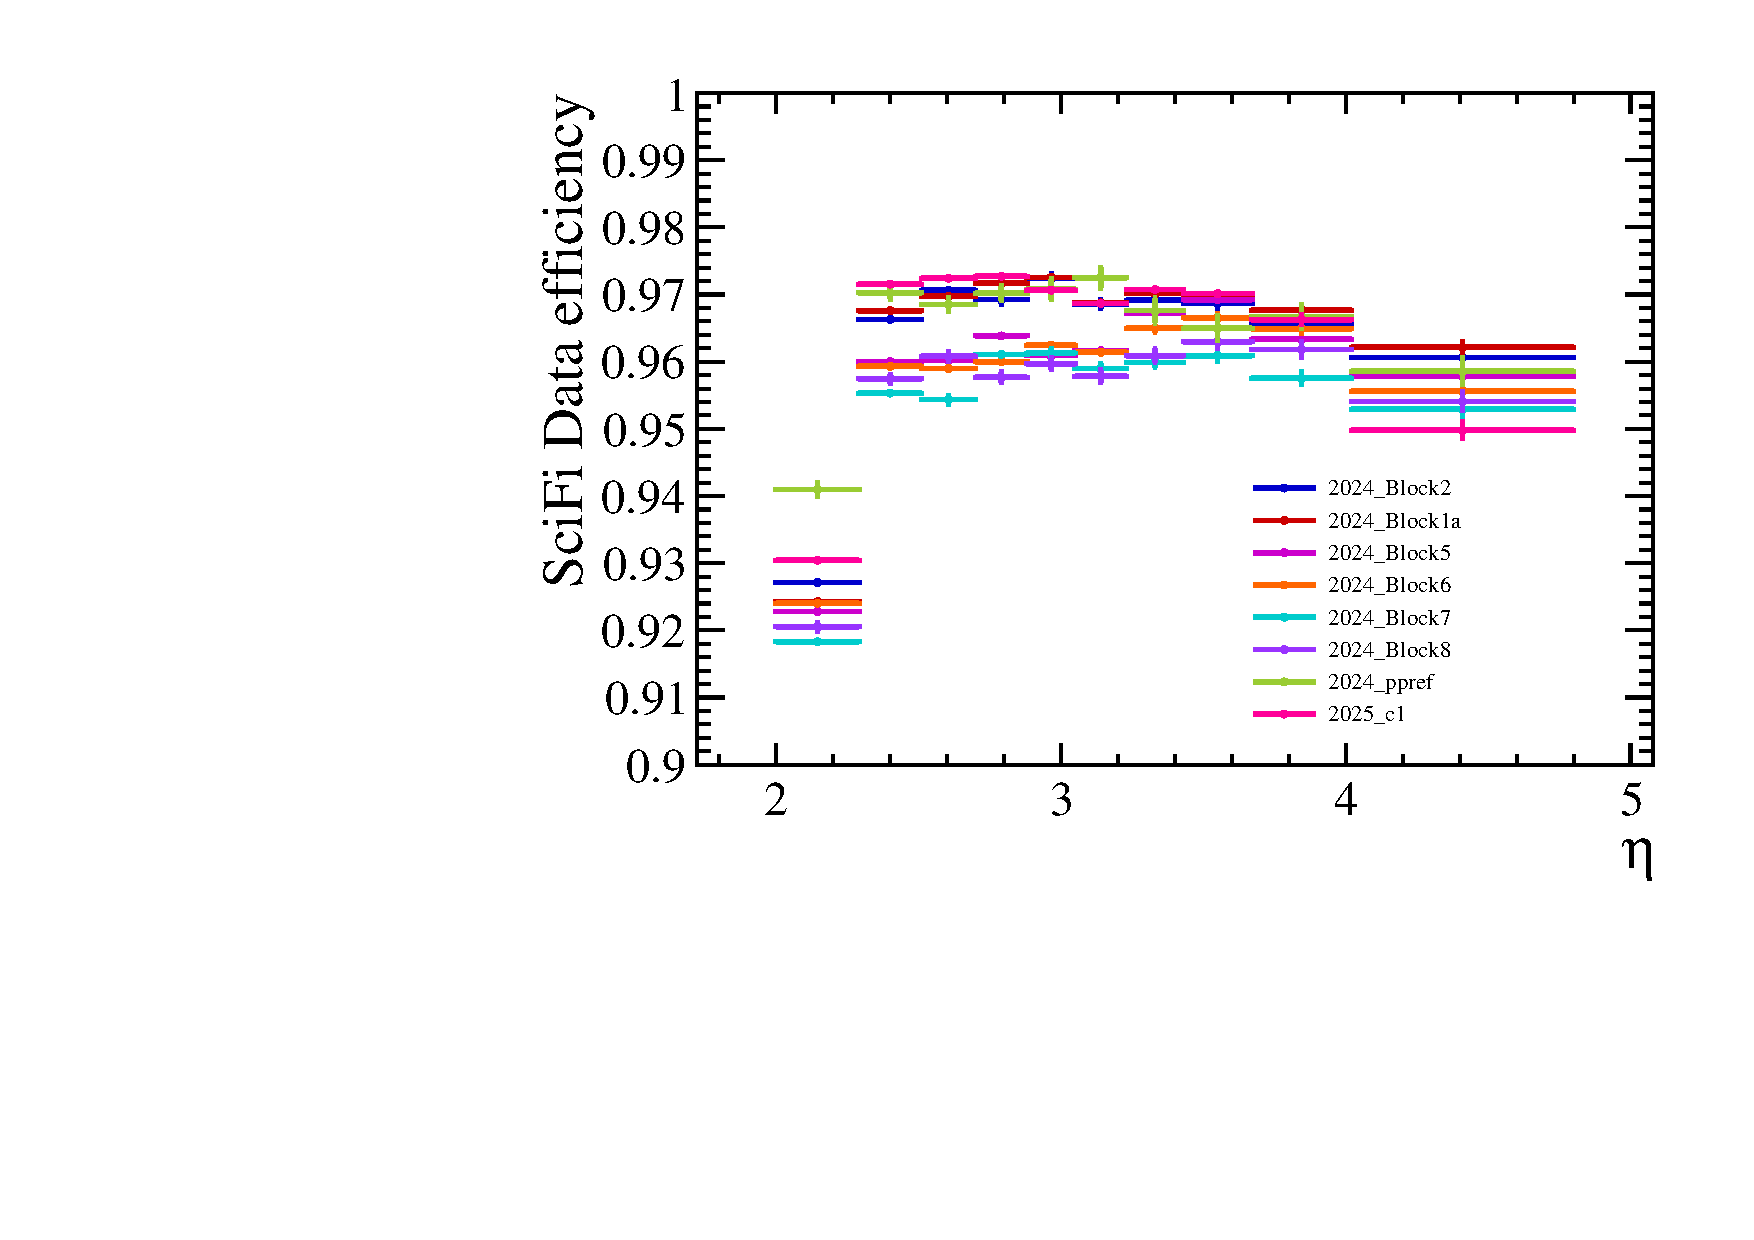
\includegraphics[width=0.75\textwidth]{Plots/trackeff_Data_VeloMuon_ETA_respruced_samples.pdf}
    \end{subfigure}
    \begin{subfigure}{0.5\textwidth}
      \centering
      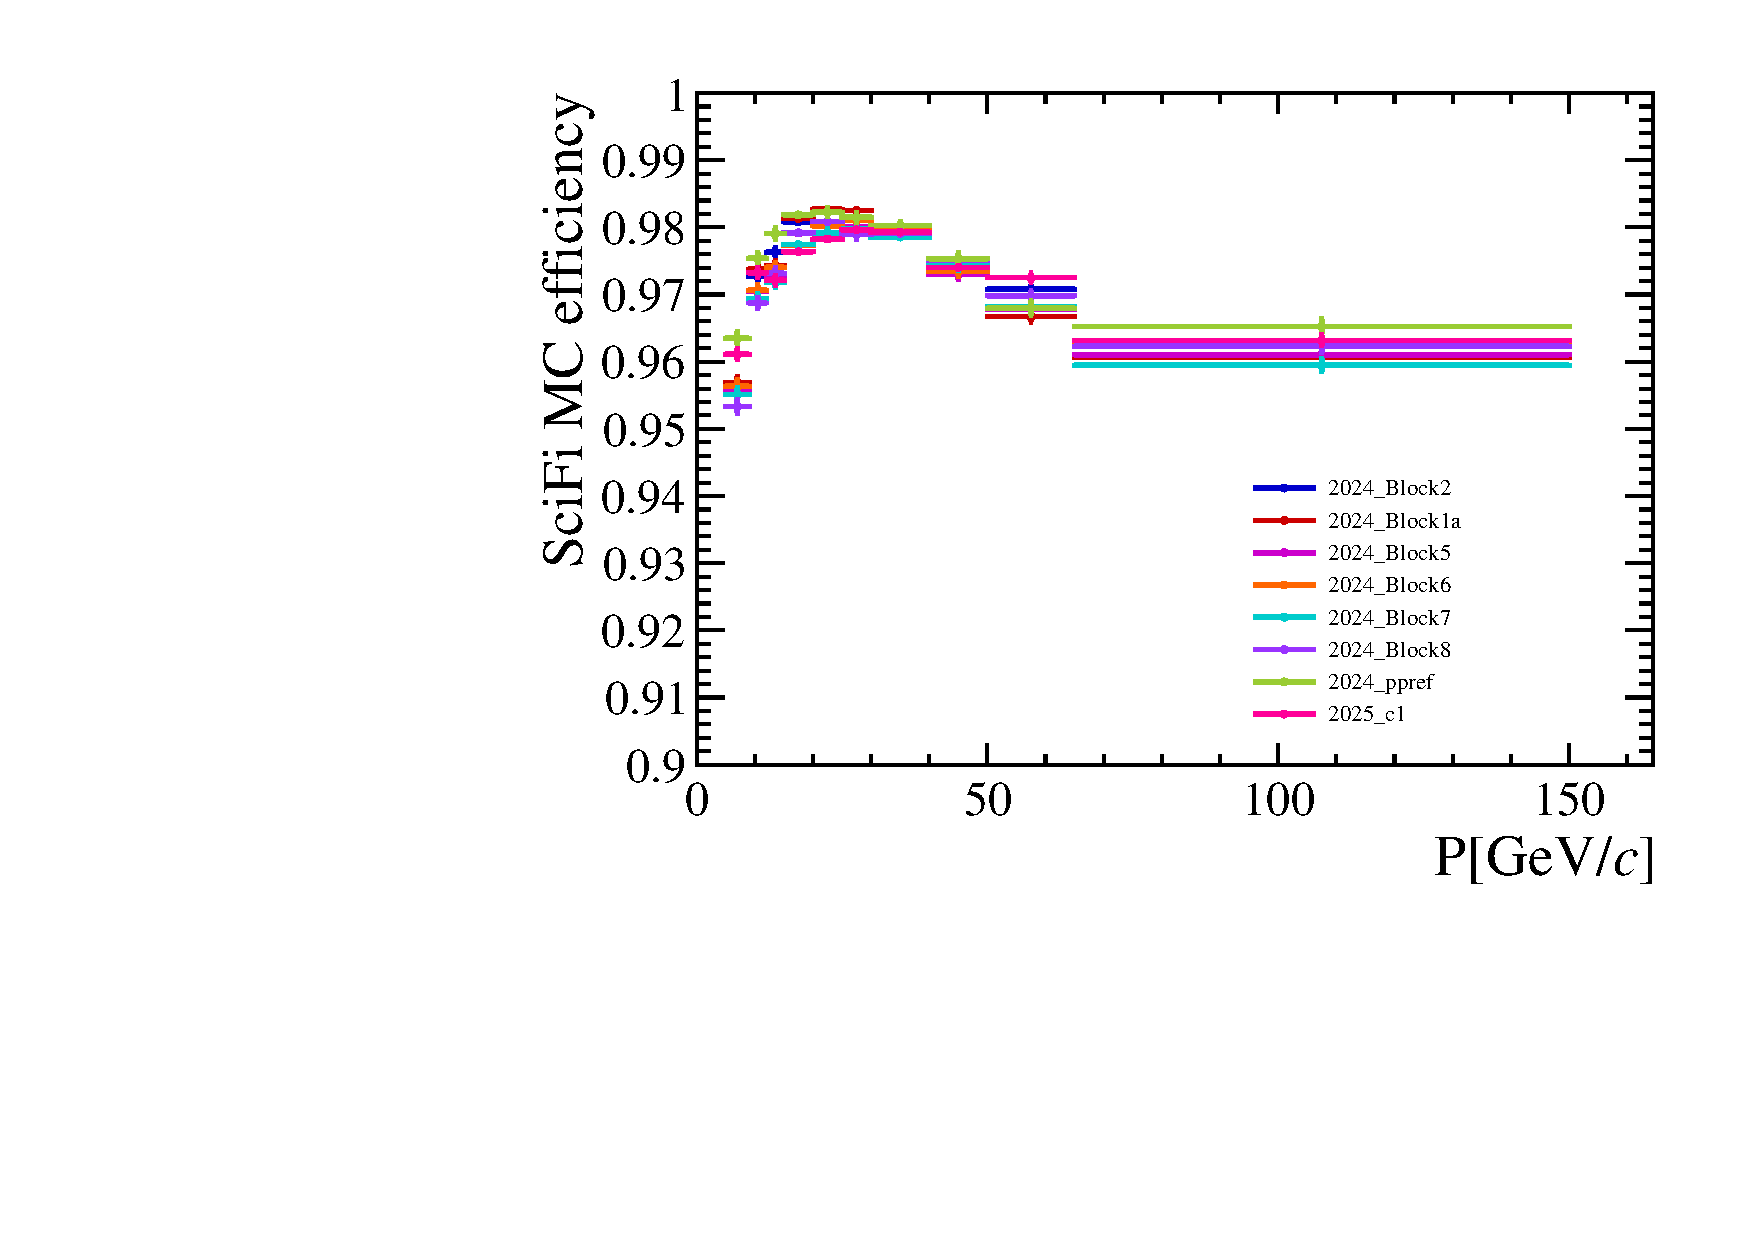
\includegraphics[width=0.75\textwidth]{Plots/trackeff_MC_VeloMuon_P_respruced_samples.pdf}
    \end{subfigure}%
    \begin{subfigure}{0.5\textwidth}
      \centering
      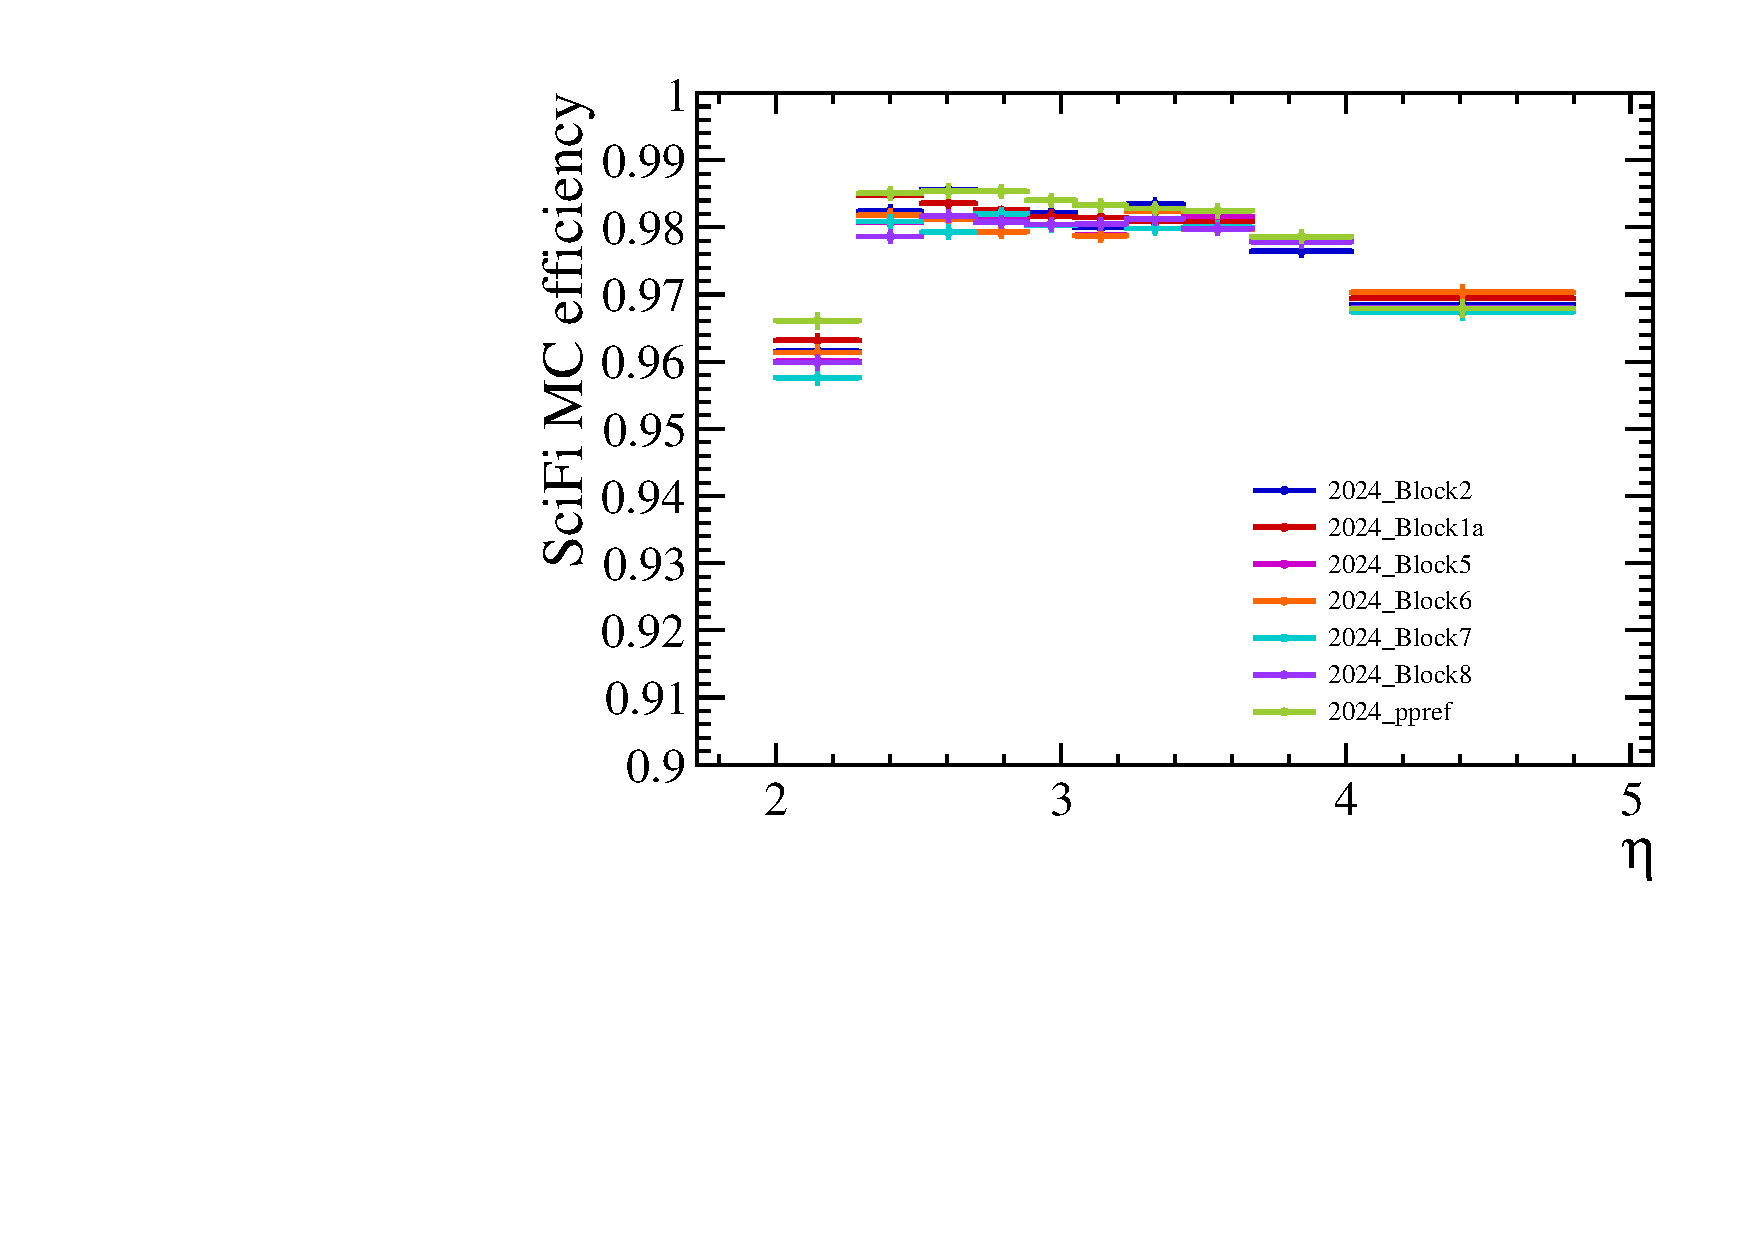
\includegraphics[width=0.75\textwidth]{Plots/trackeff_MC_VeloMuon_ETA_respruced_samples.pdf}
    \end{subfigure}
  \end{figure}
\end{frame}

\begin{frame}{Efficiency comparisons}
  \vspace{0.0cm}
  {\large Comparison of Velo tracking efficiencies in all data blocks}
  \begin{figure}[htb]
    \centering
    \begin{subfigure}{0.5\textwidth}
      \centering
      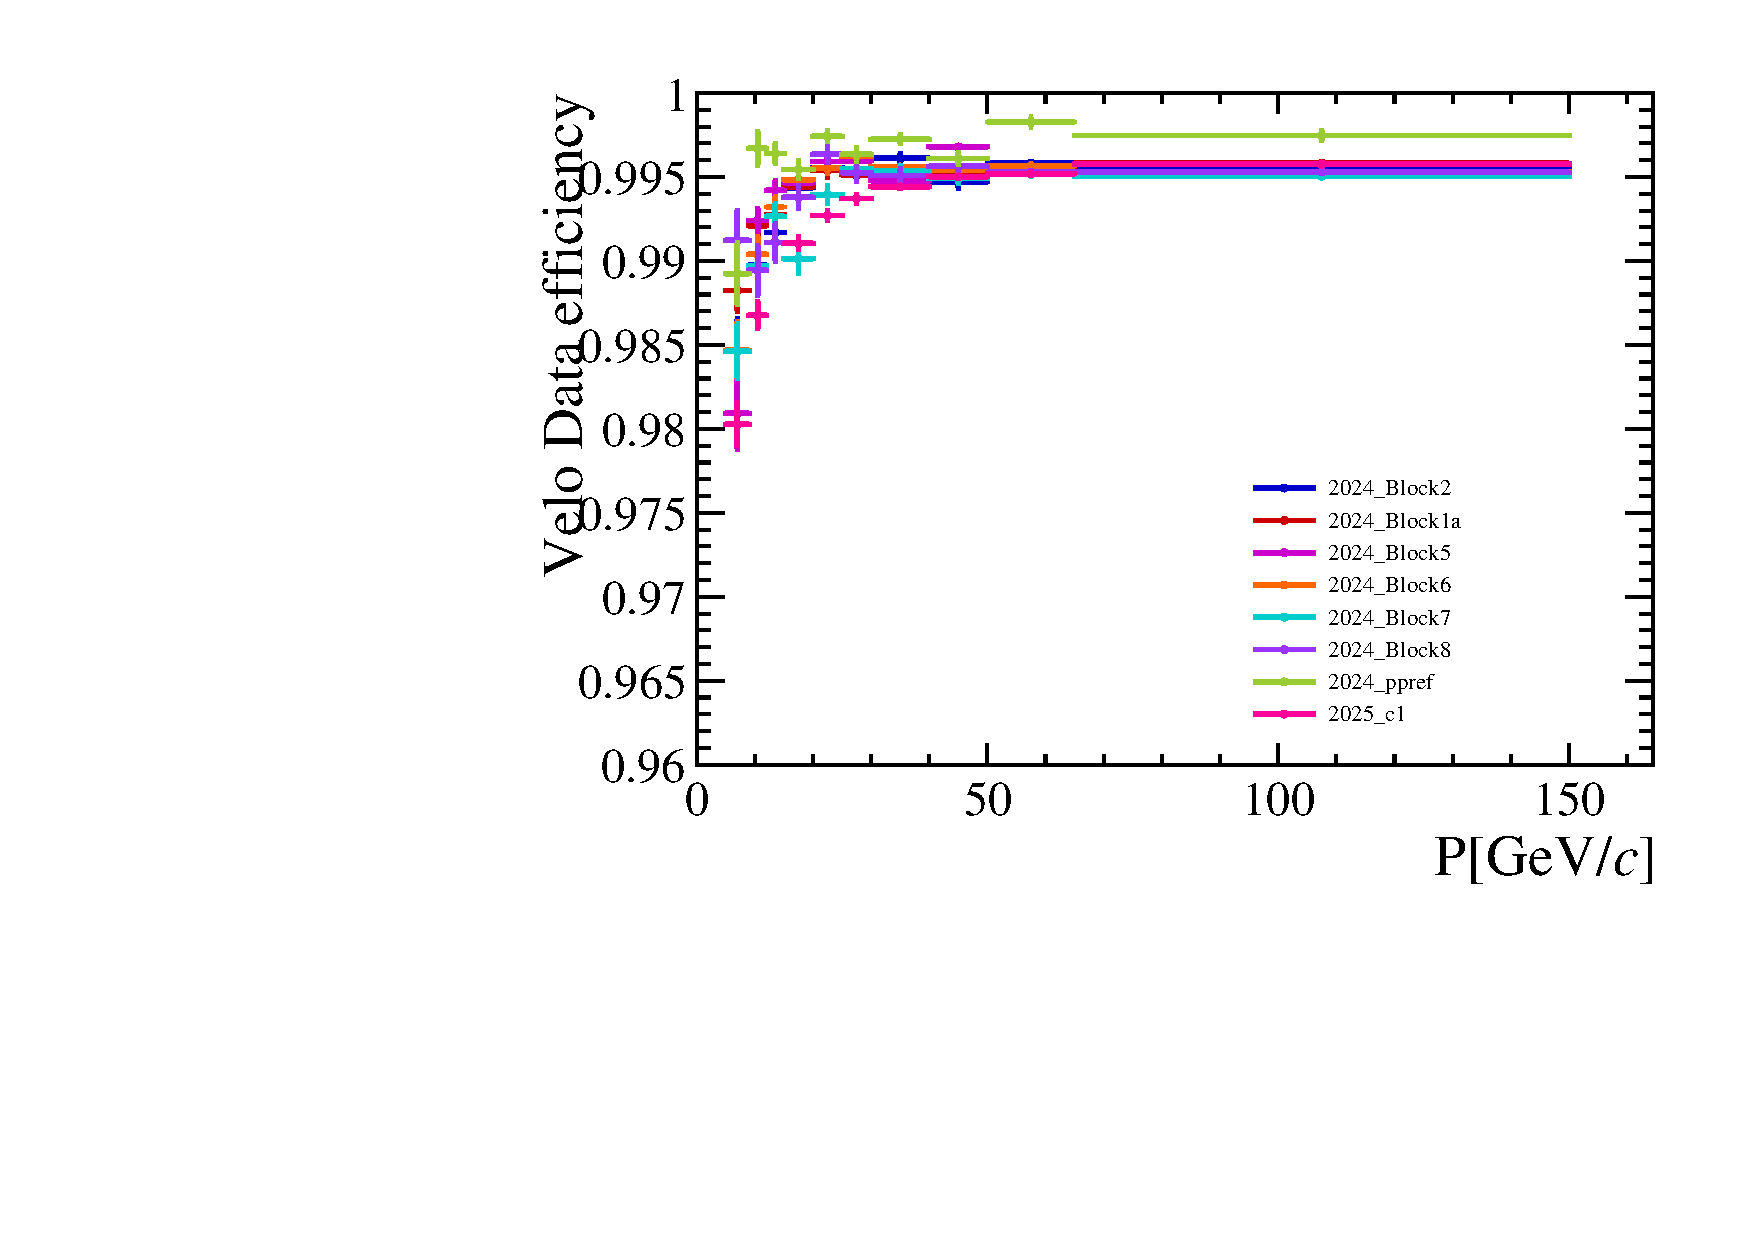
\includegraphics[width=0.75\textwidth]{Plots/trackeff_Data_Downstream_P_respruced_samples.pdf}
    \end{subfigure}%
    \begin{subfigure}{0.5\textwidth}
      \centering
      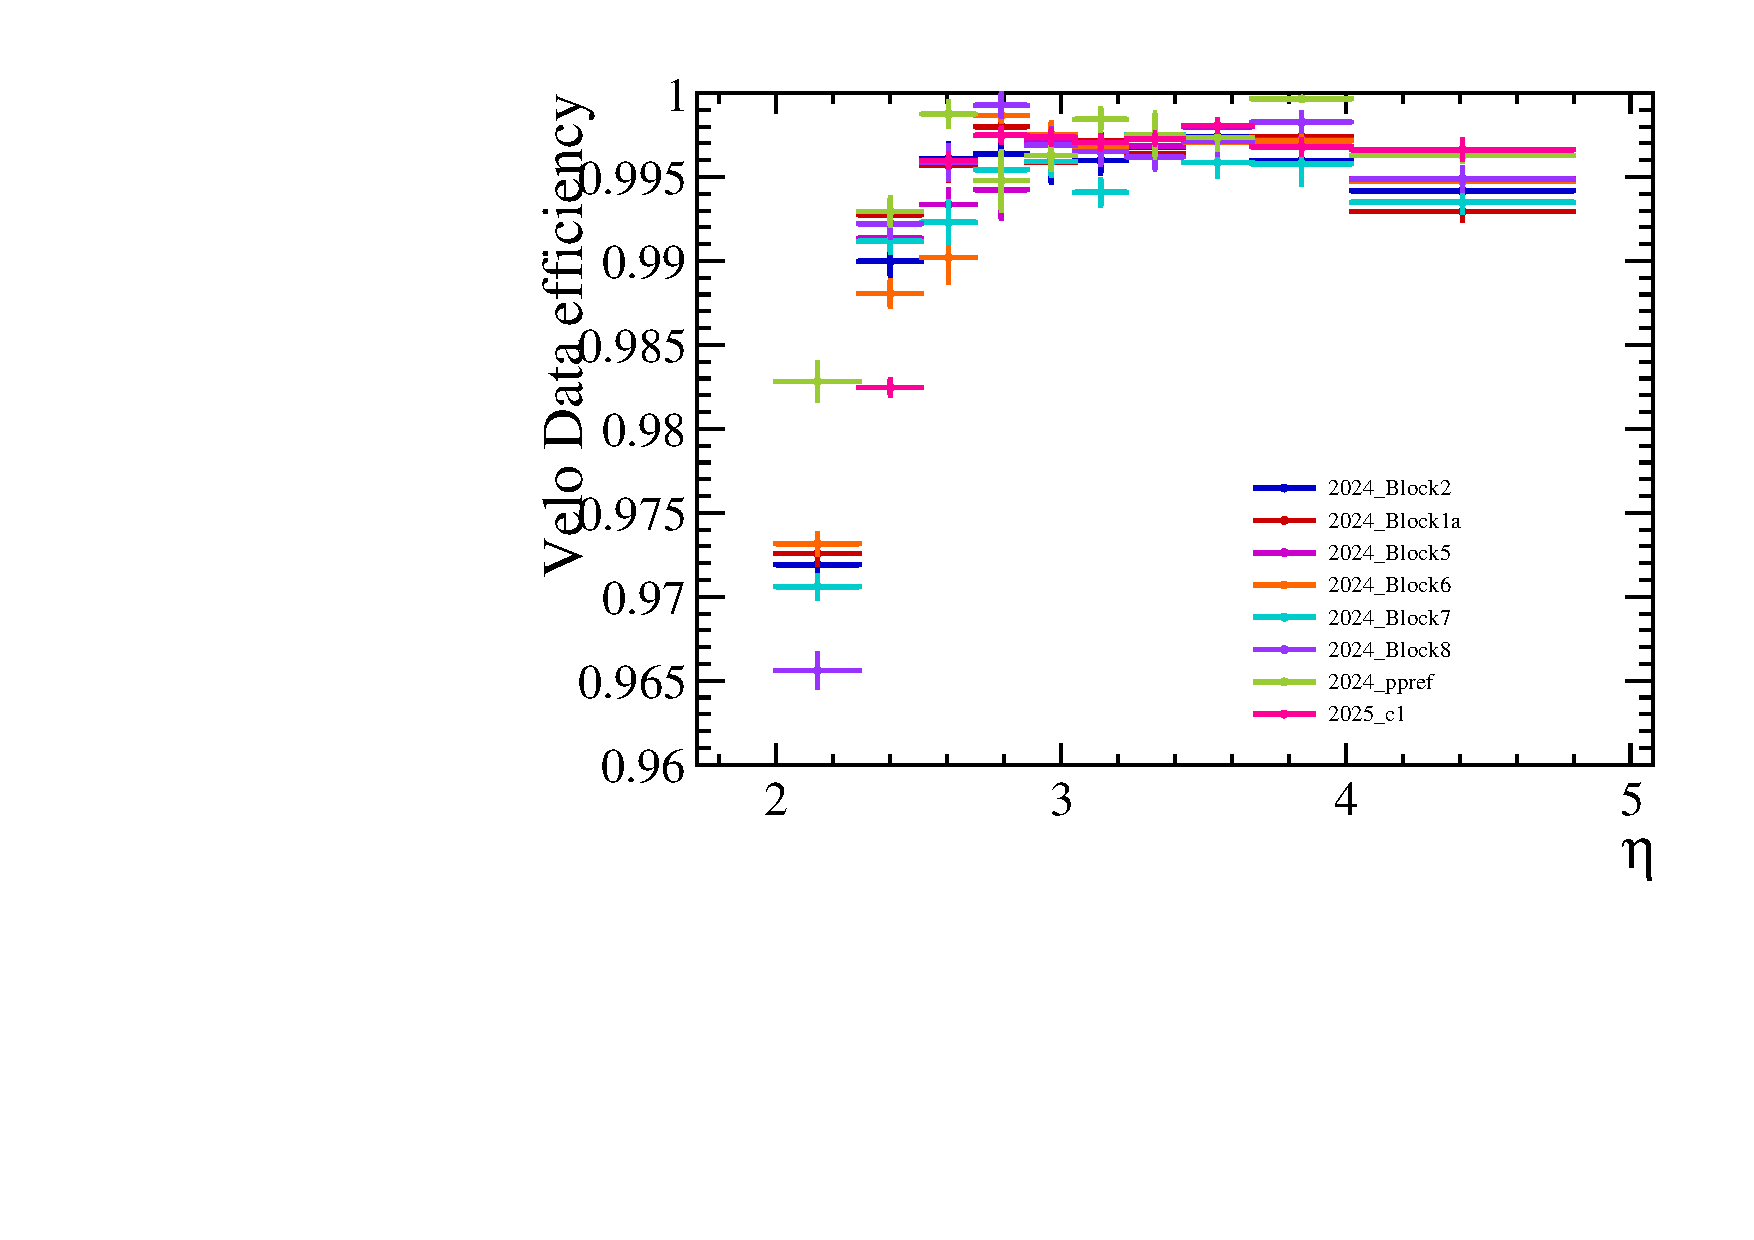
\includegraphics[width=0.75\textwidth]{Plots/trackeff_Data_Downstream_ETA_respruced_samples.pdf}
    \end{subfigure}
    \begin{subfigure}{0.5\textwidth}
      \centering
      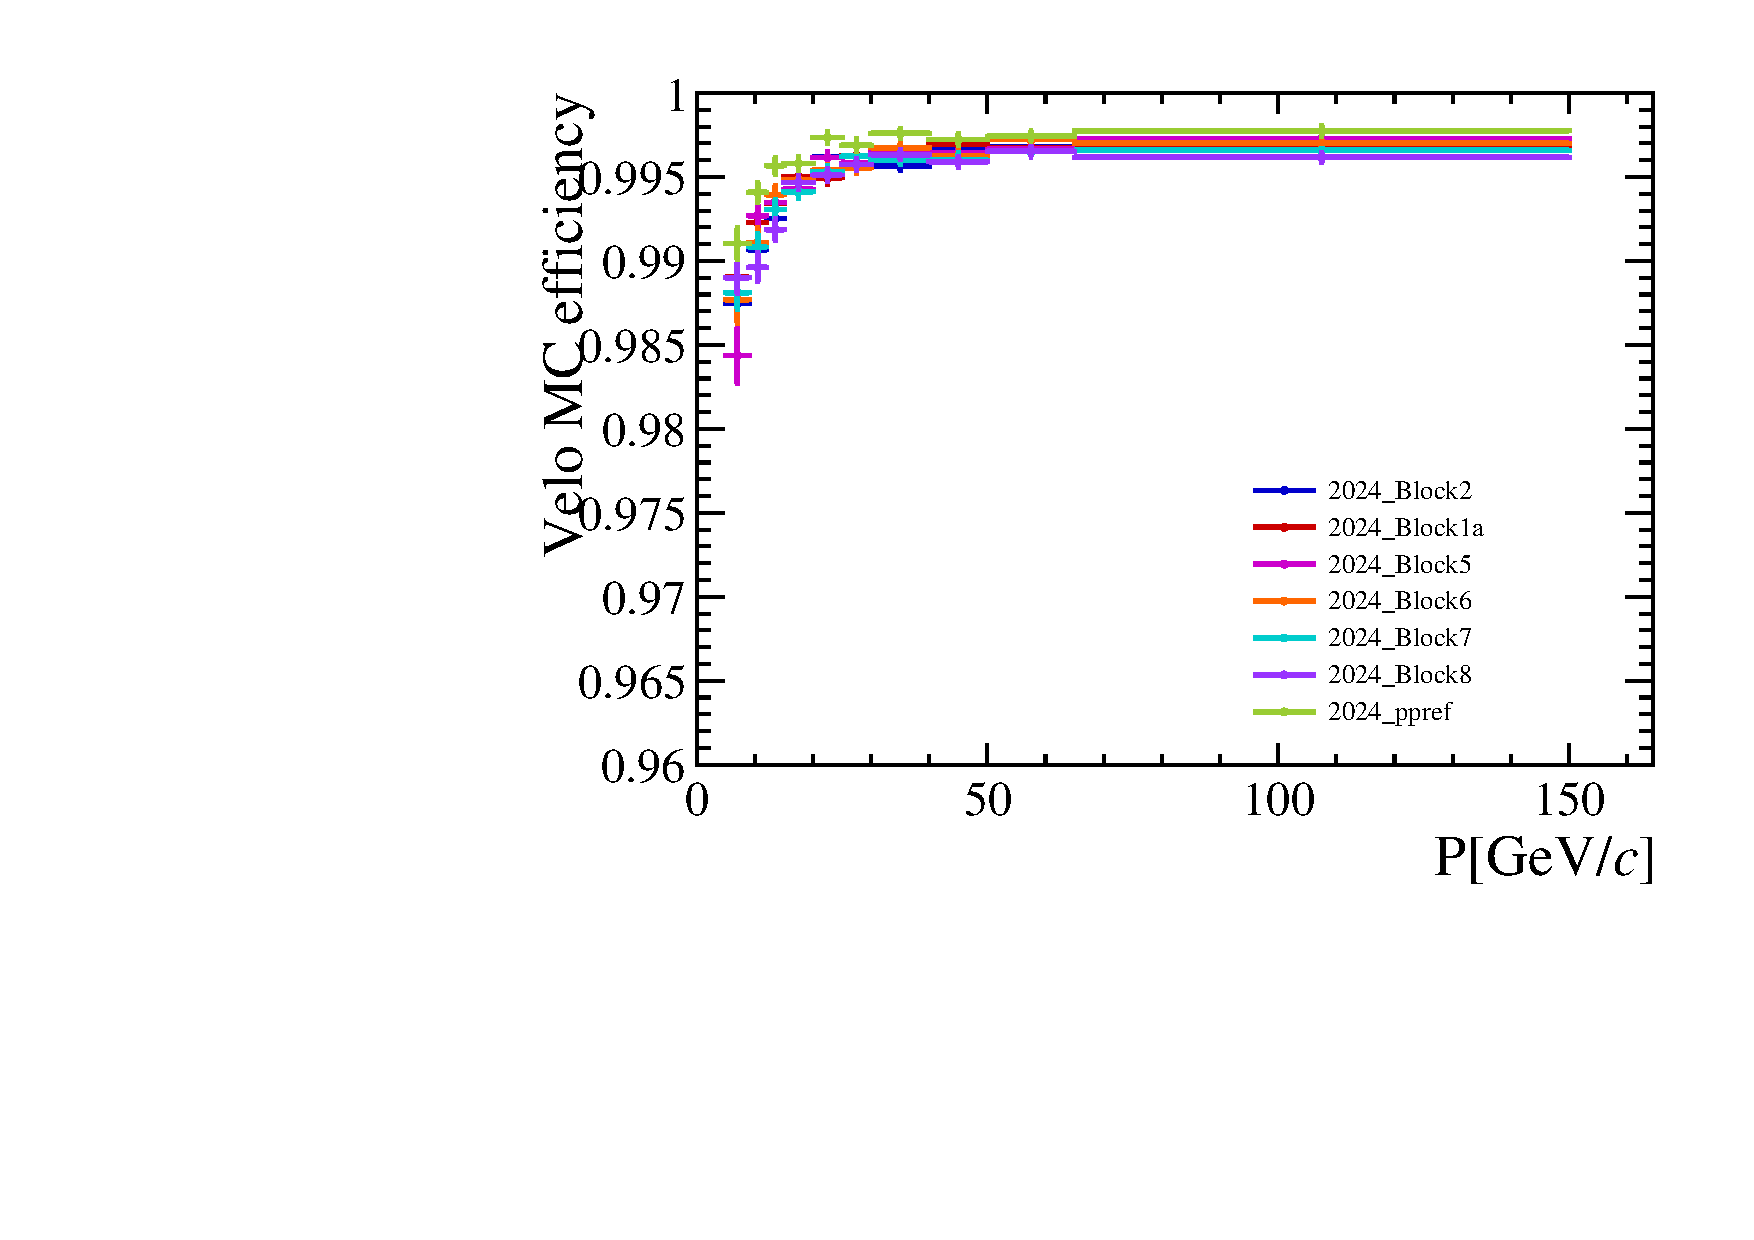
\includegraphics[width=0.75\textwidth]{Plots/trackeff_MC_Downstream_P_respruced_samples.pdf}
    \end{subfigure}%
    \begin{subfigure}{0.5\textwidth}
      \centering
      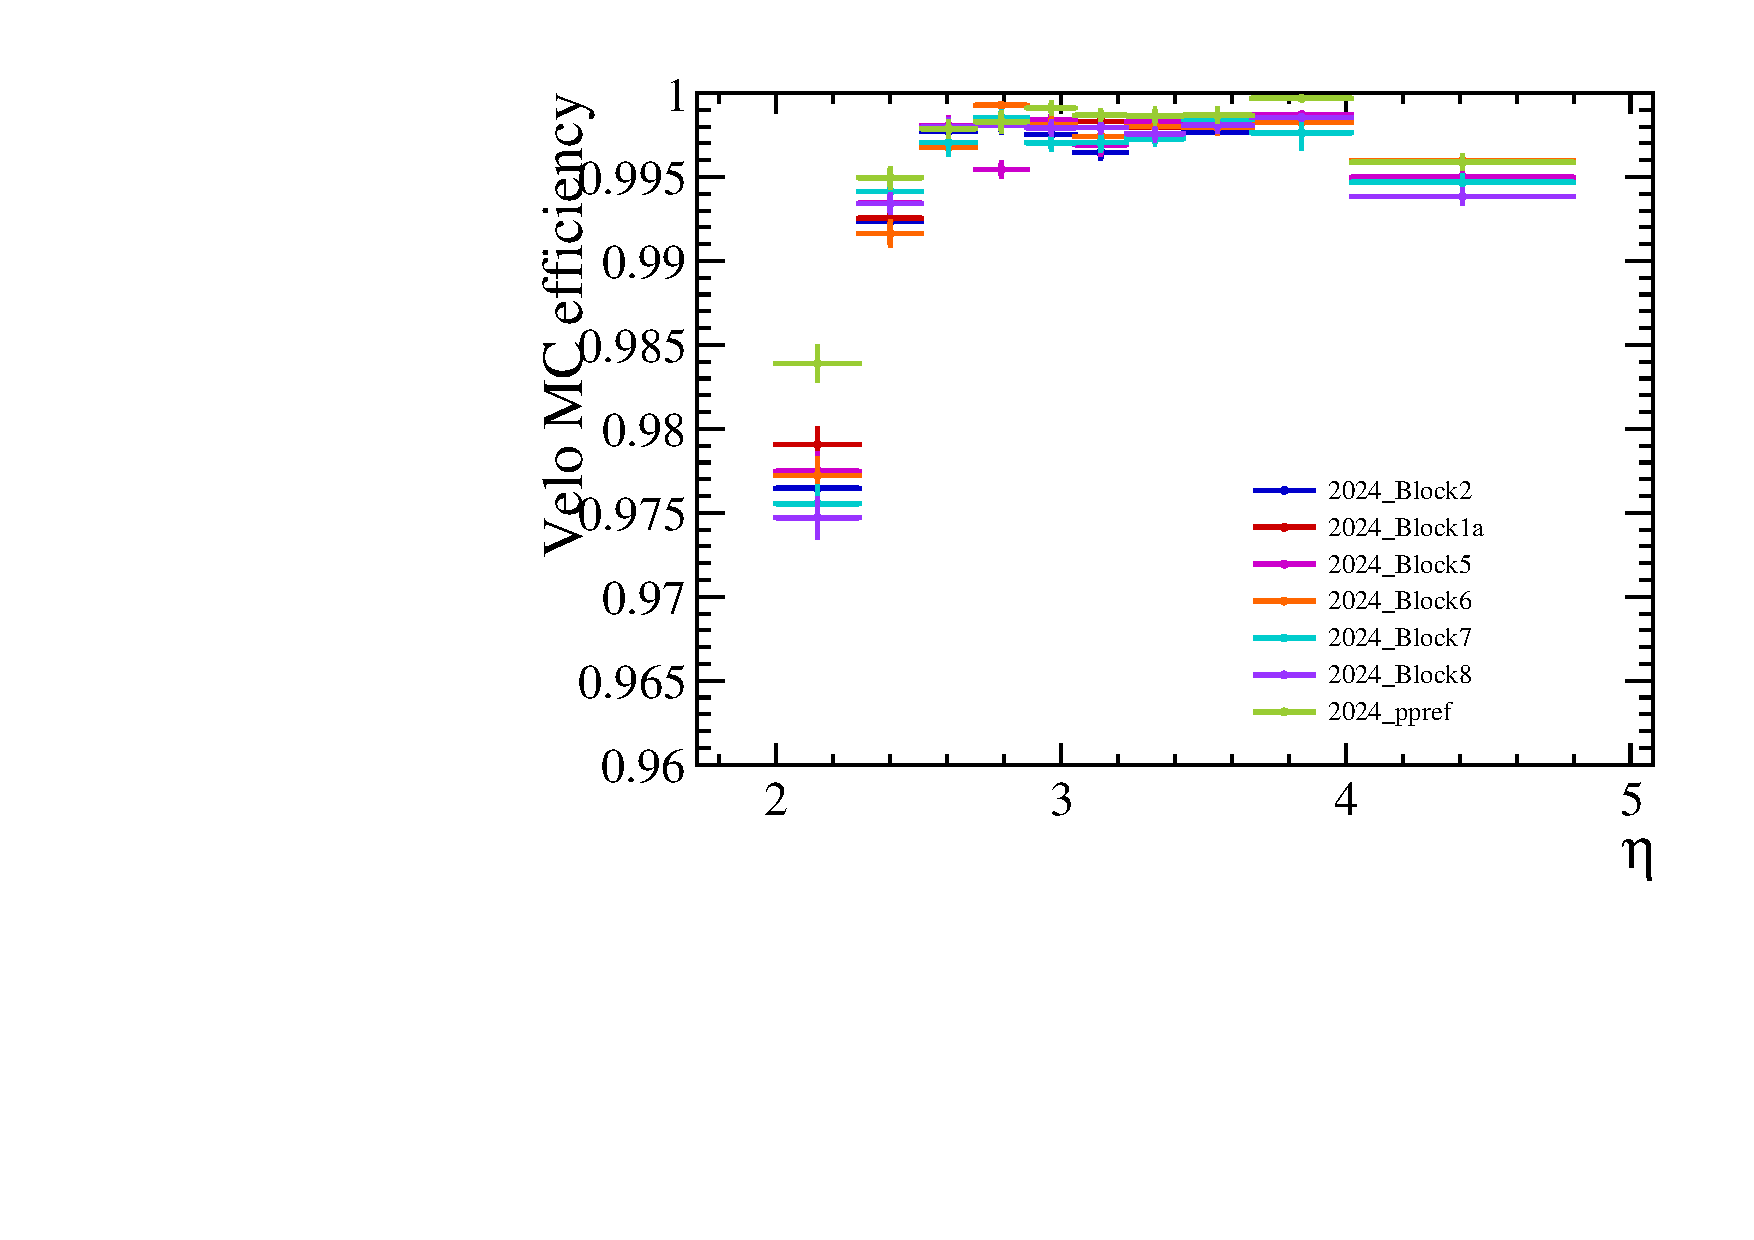
\includegraphics[width=0.75\textwidth]{Plots/trackeff_MC_Downstream_ETA_respruced_samples.pdf}
    \end{subfigure}
  \end{figure}
\end{frame}

\begin{frame}{Efficiency comparisons}
  \vspace{0.0cm}
  {\large 2025 Data-MC discrepancy}
  \begin{figure}[htb]
    \centering
    \begin{subfigure}{0.5\textwidth}
      \centering
      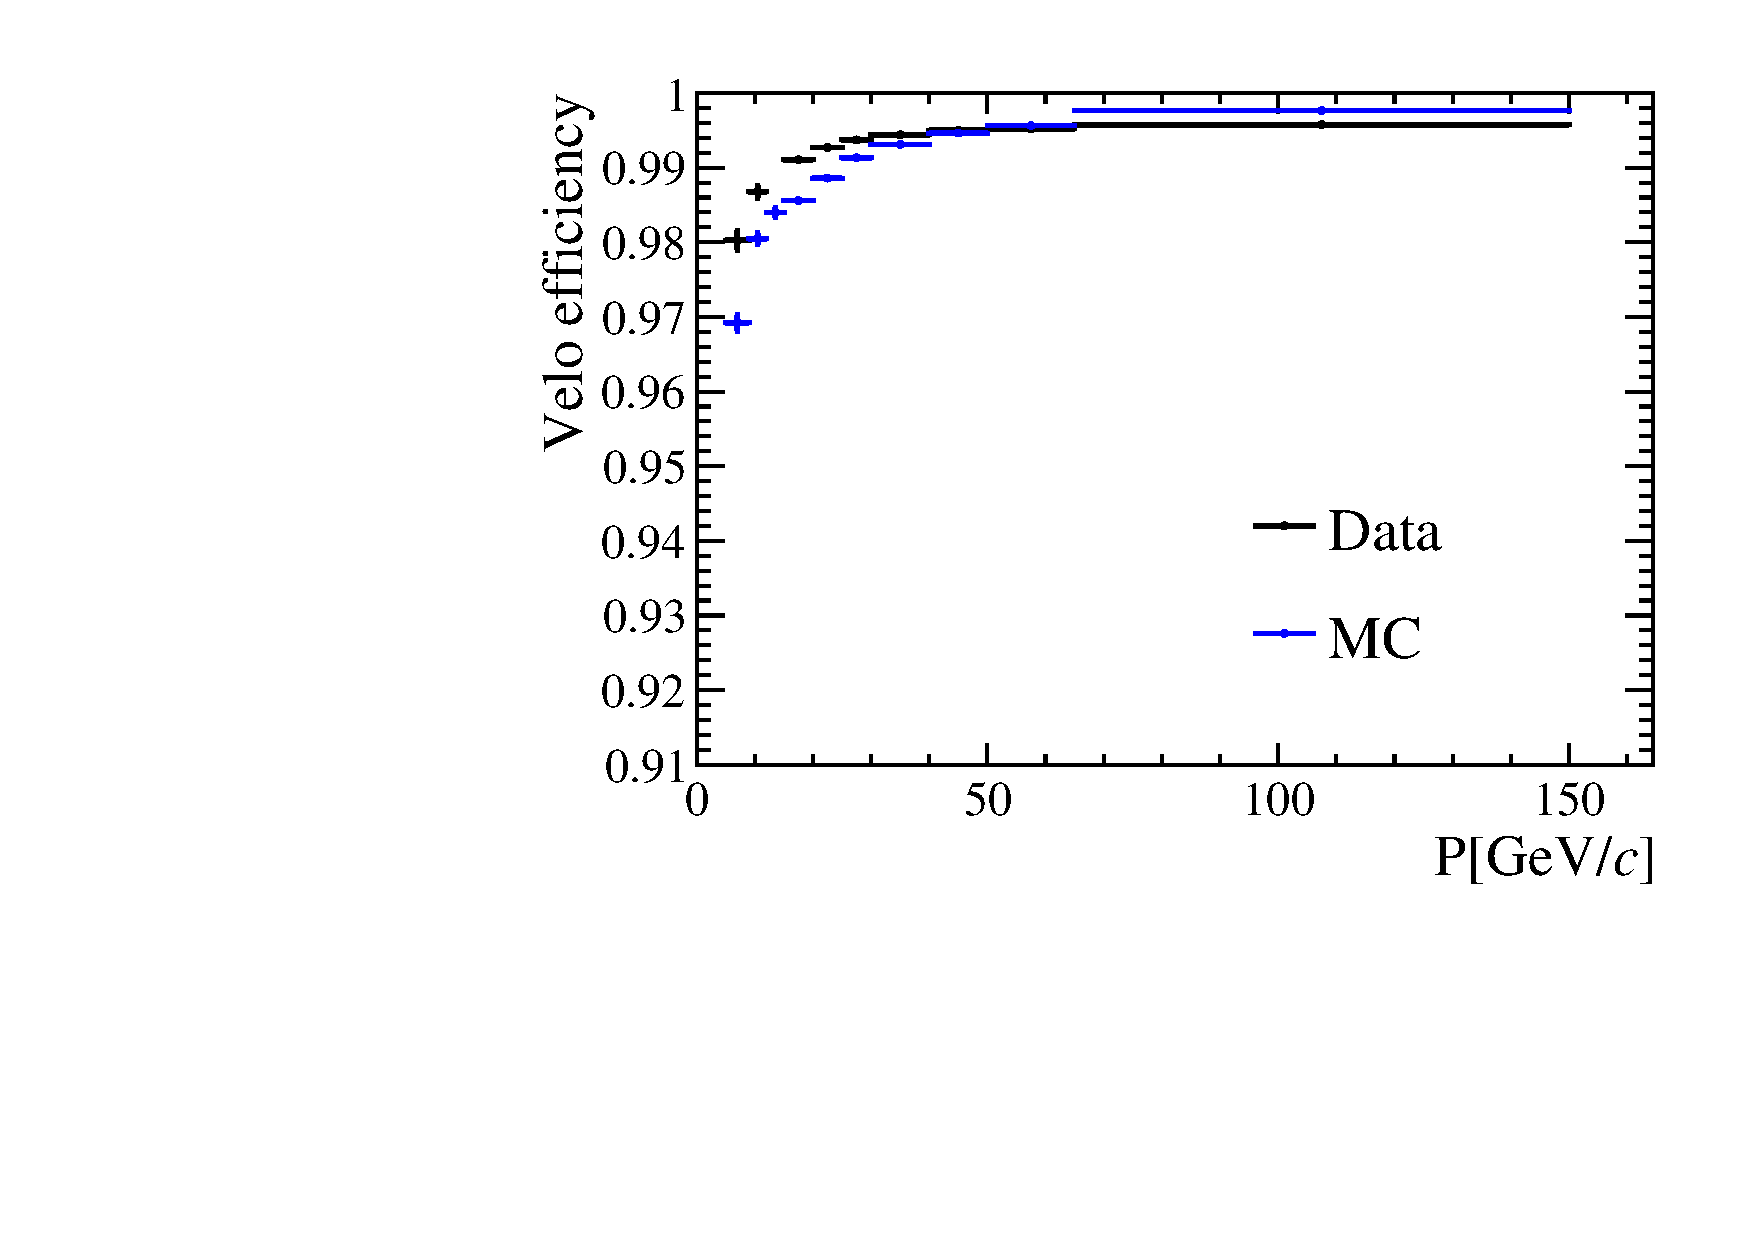
\includegraphics[width=1.0\textwidth]{Plots/trackeff_Downstream_P_2025_c1_Data_MC_samples.pdf}
    \end{subfigure}%
    \begin{subfigure}{0.5\textwidth}
      \centering
      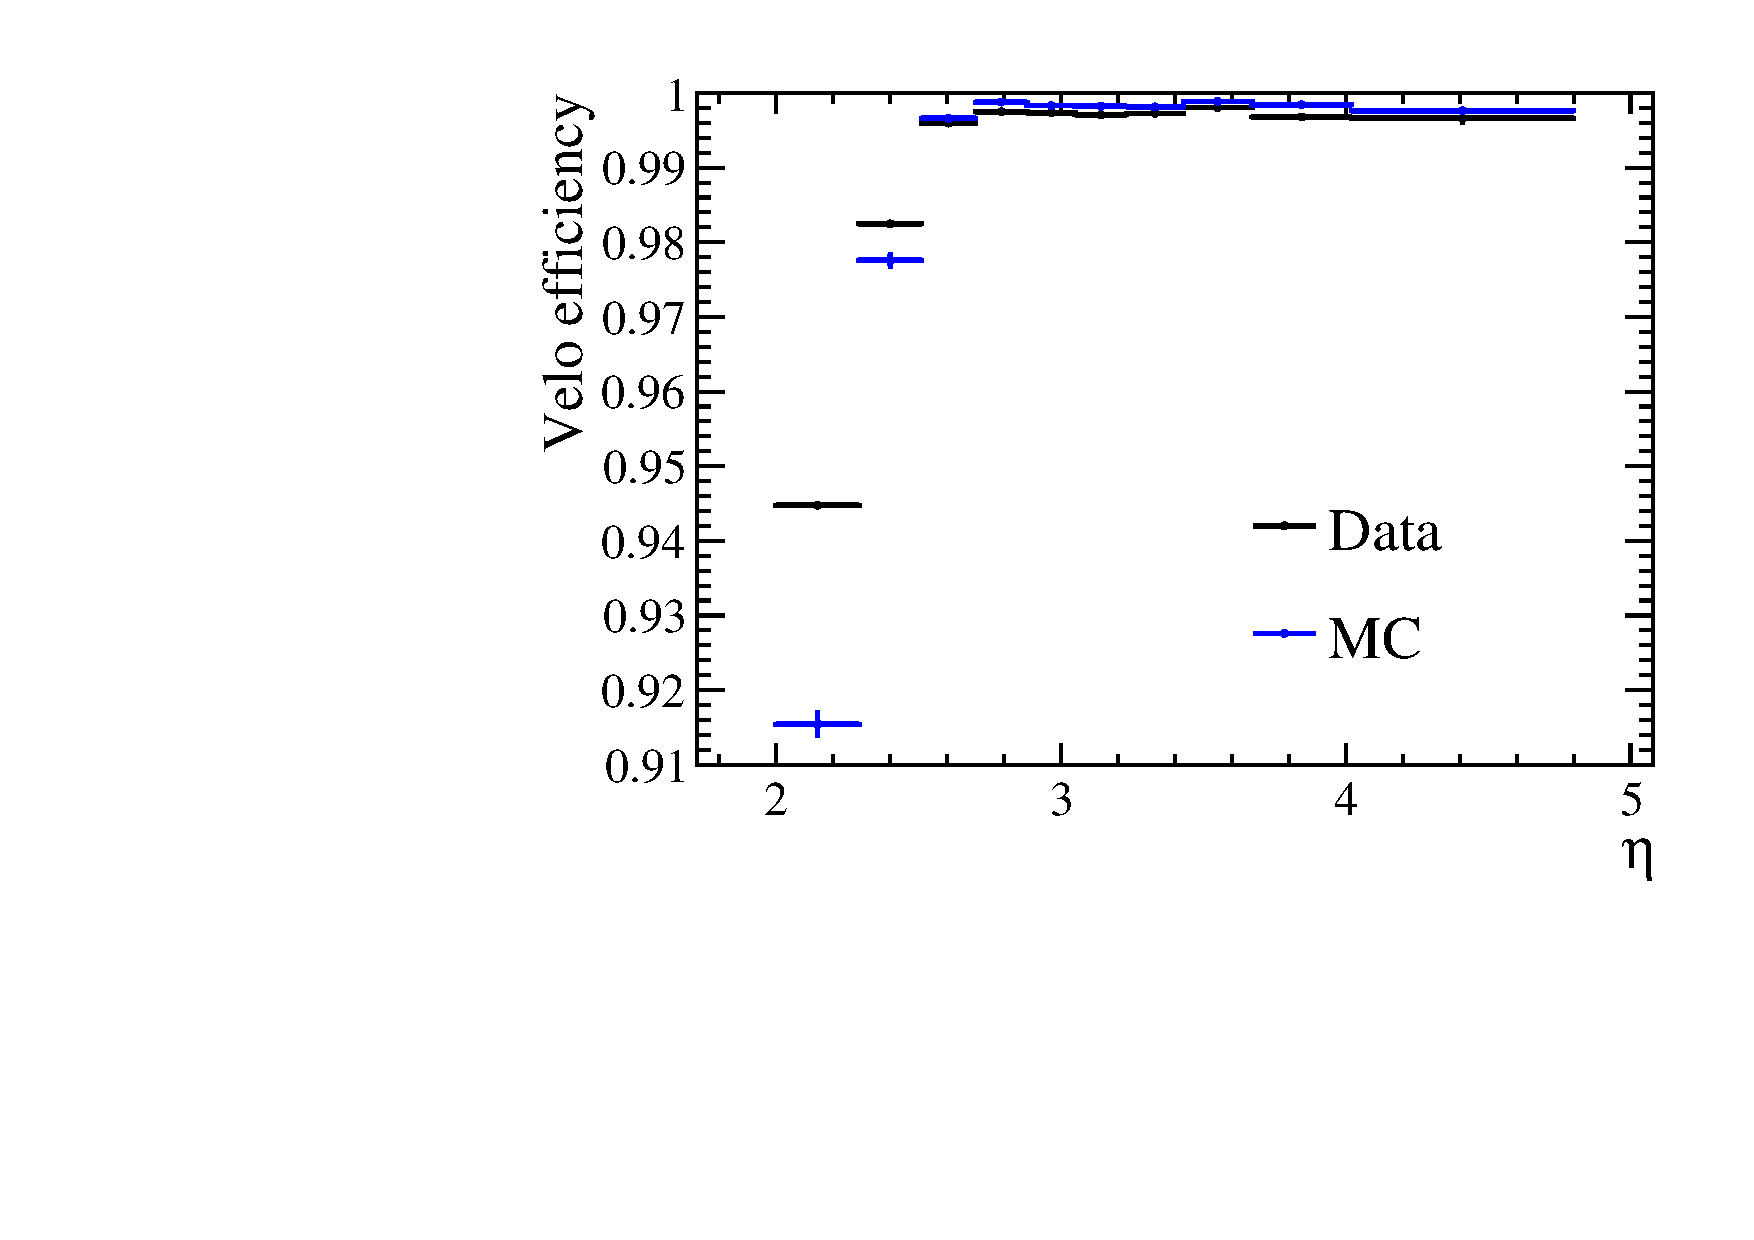
\includegraphics[width=1.0\textwidth]{Plots/trackeff_Downstream_ETA_2025_c1_Data_MC_samples.pdf}
    \end{subfigure}
  \end{figure}
  {Need to understand why MC underestimates the Velo efficiency in 2025!}
\end{frame}

\begin{frame}{Efficiency comparisons}
  \vspace{0.0cm}
  {\large Comparison of long (MuonUT) tracking efficiencies in all data blocks}
  \begin{figure}[htb]
    \centering
    \begin{subfigure}{0.5\textwidth}
      \centering
      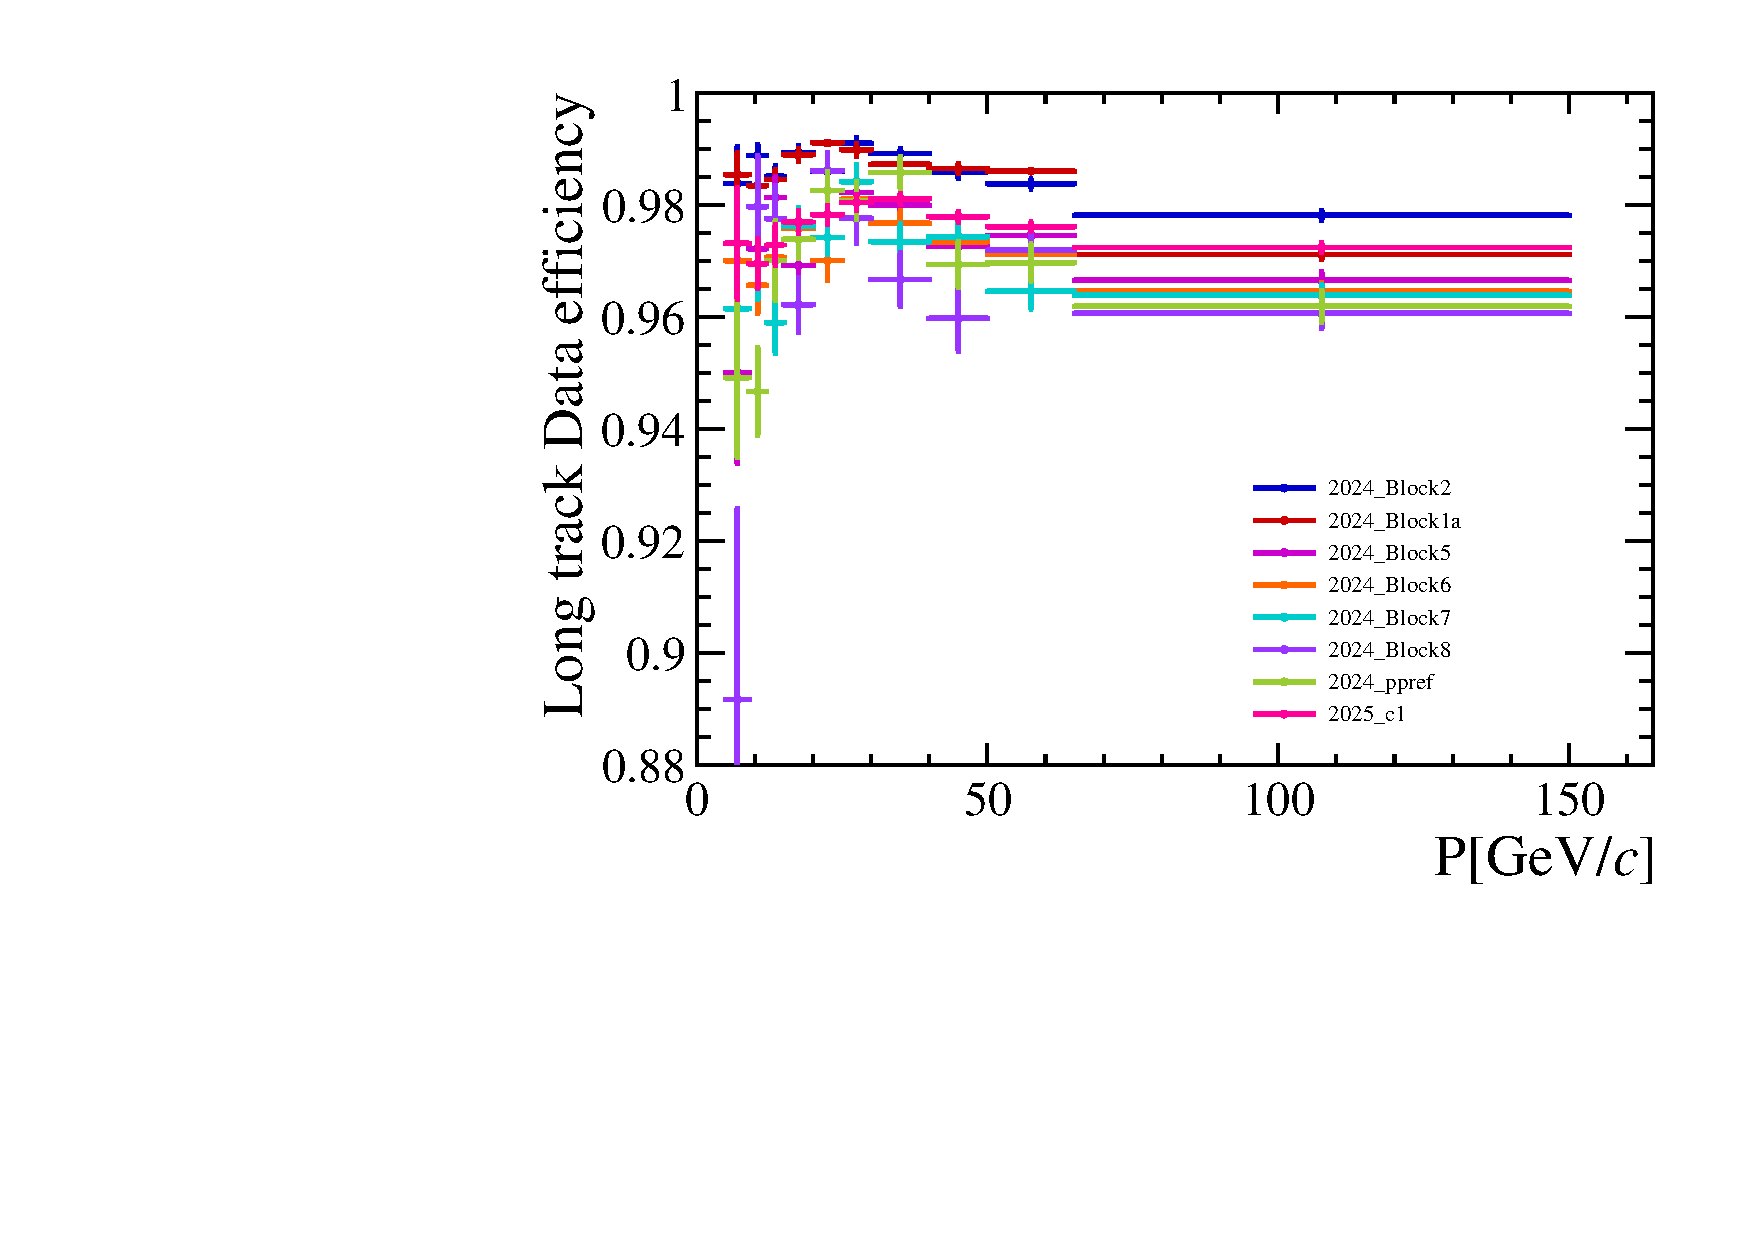
\includegraphics[width=0.75\textwidth]{Plots/trackeff_Data_MuonUT_P_respruced_samples.pdf}
    \end{subfigure}%
    \begin{subfigure}{0.5\textwidth}
      \centering
      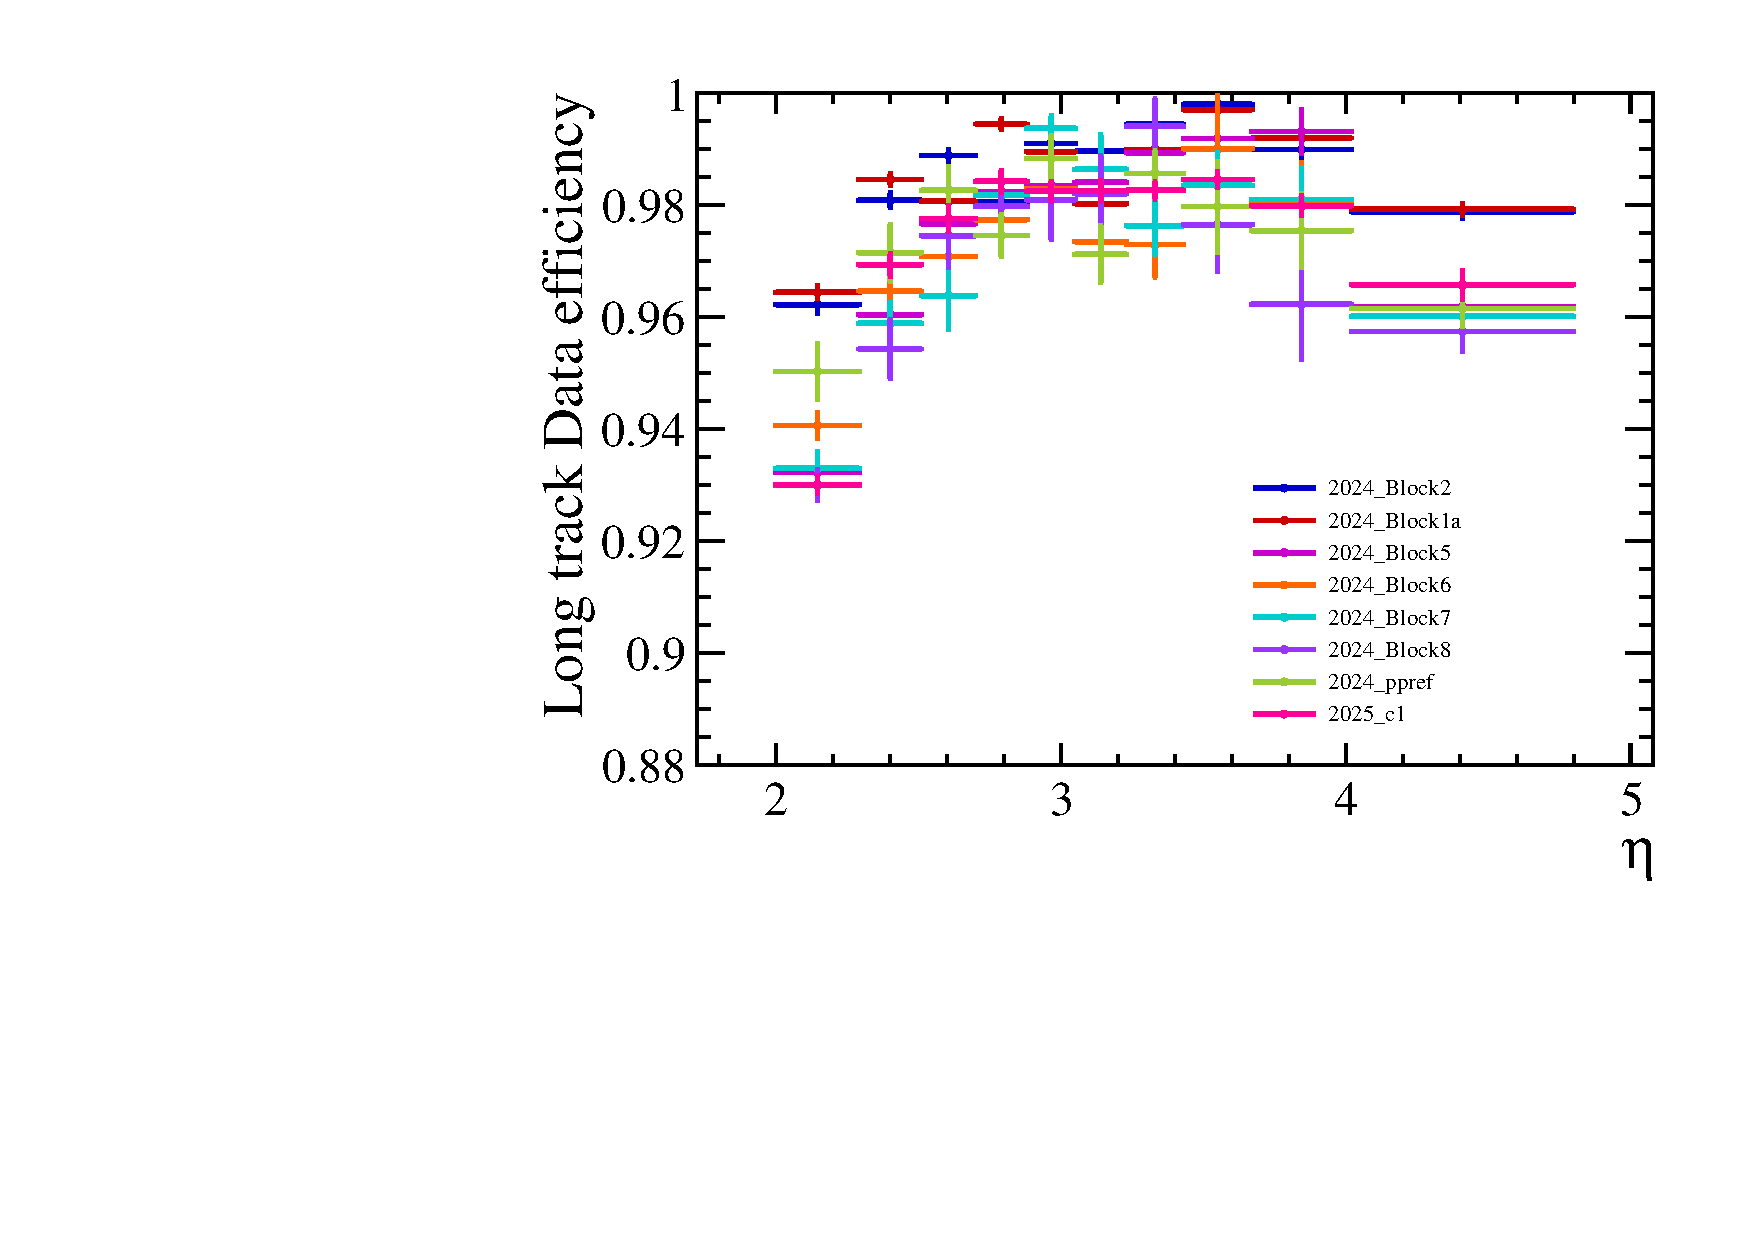
\includegraphics[width=0.75\textwidth]{Plots/trackeff_Data_MuonUT_ETA_respruced_samples.pdf}
    \end{subfigure}
    \begin{subfigure}{0.5\textwidth}
      \centering
      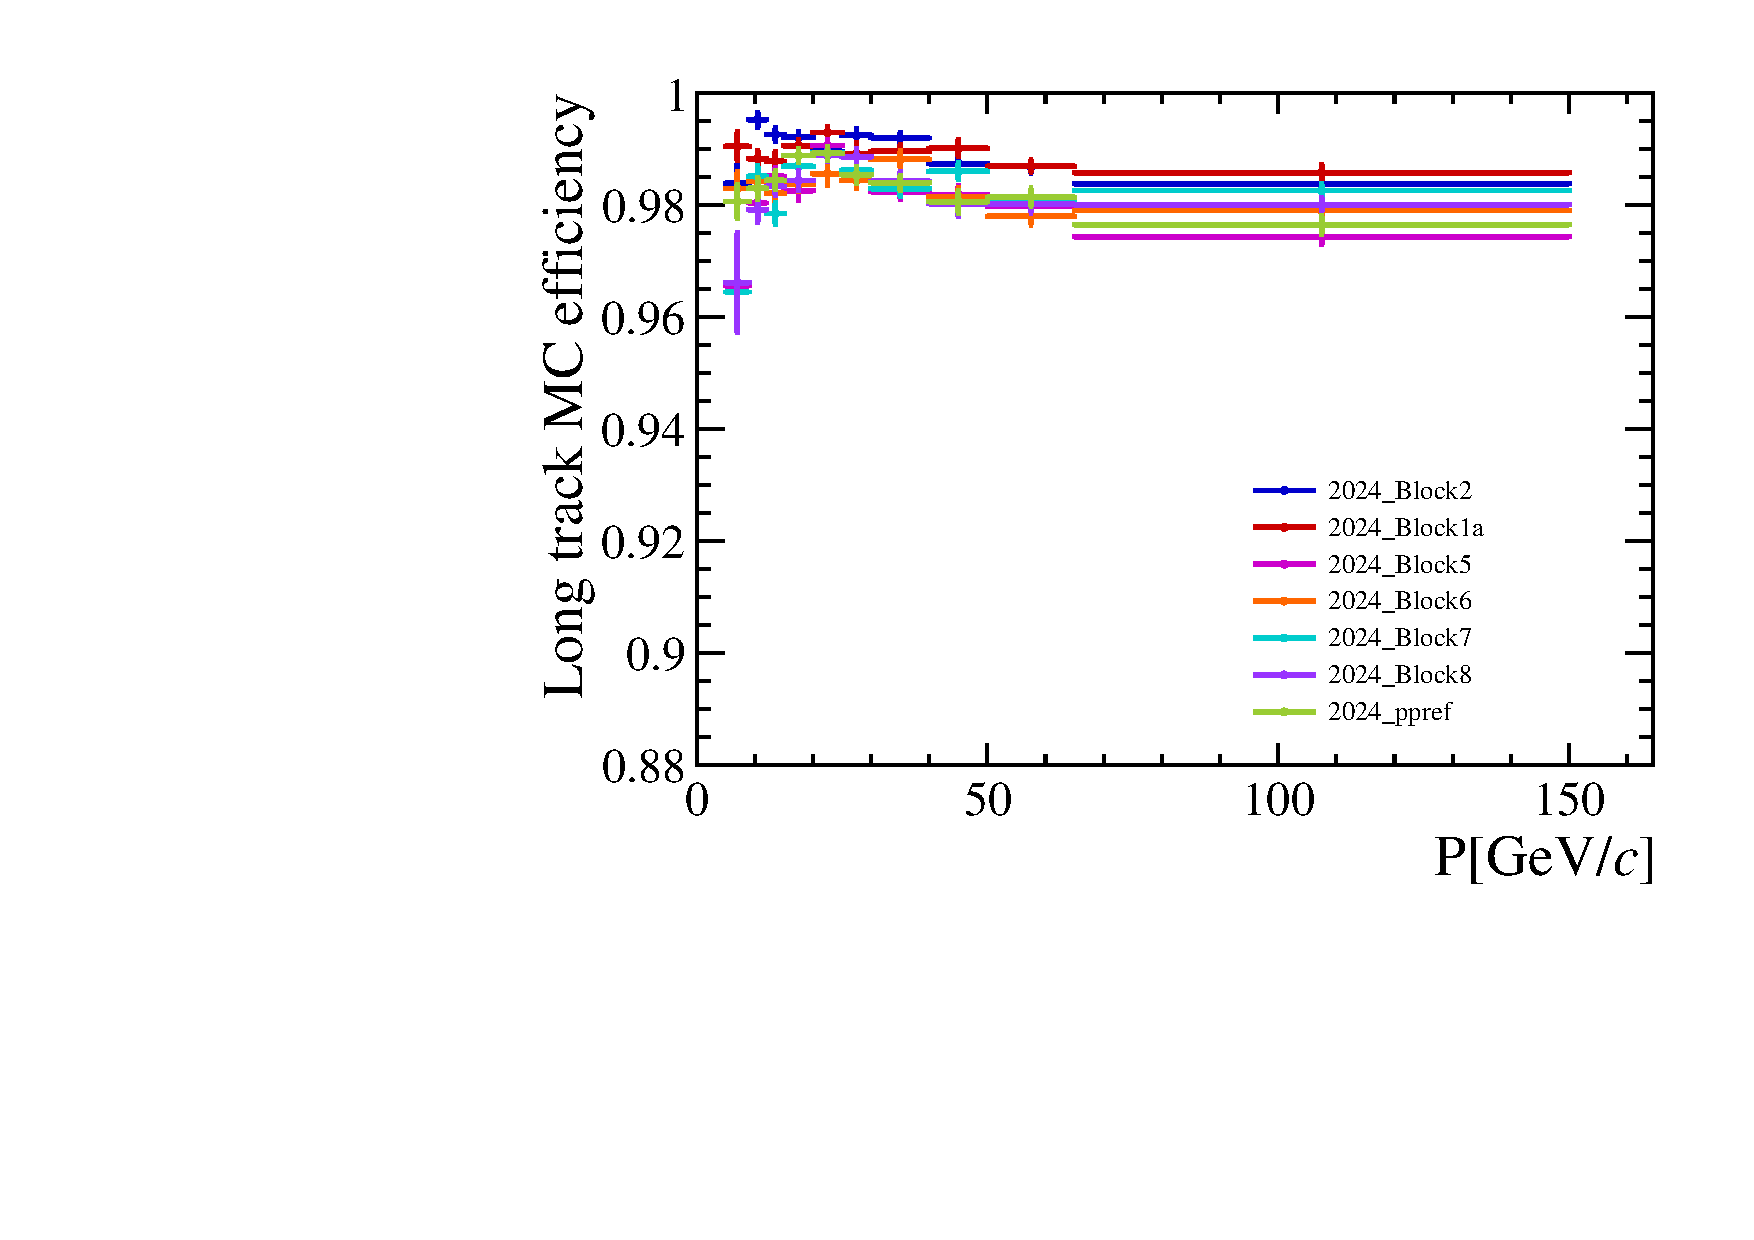
\includegraphics[width=0.75\textwidth]{Plots/trackeff_MC_MuonUT_P_respruced_samples.pdf}
    \end{subfigure}%
    \begin{subfigure}{0.5\textwidth}
      \centering
      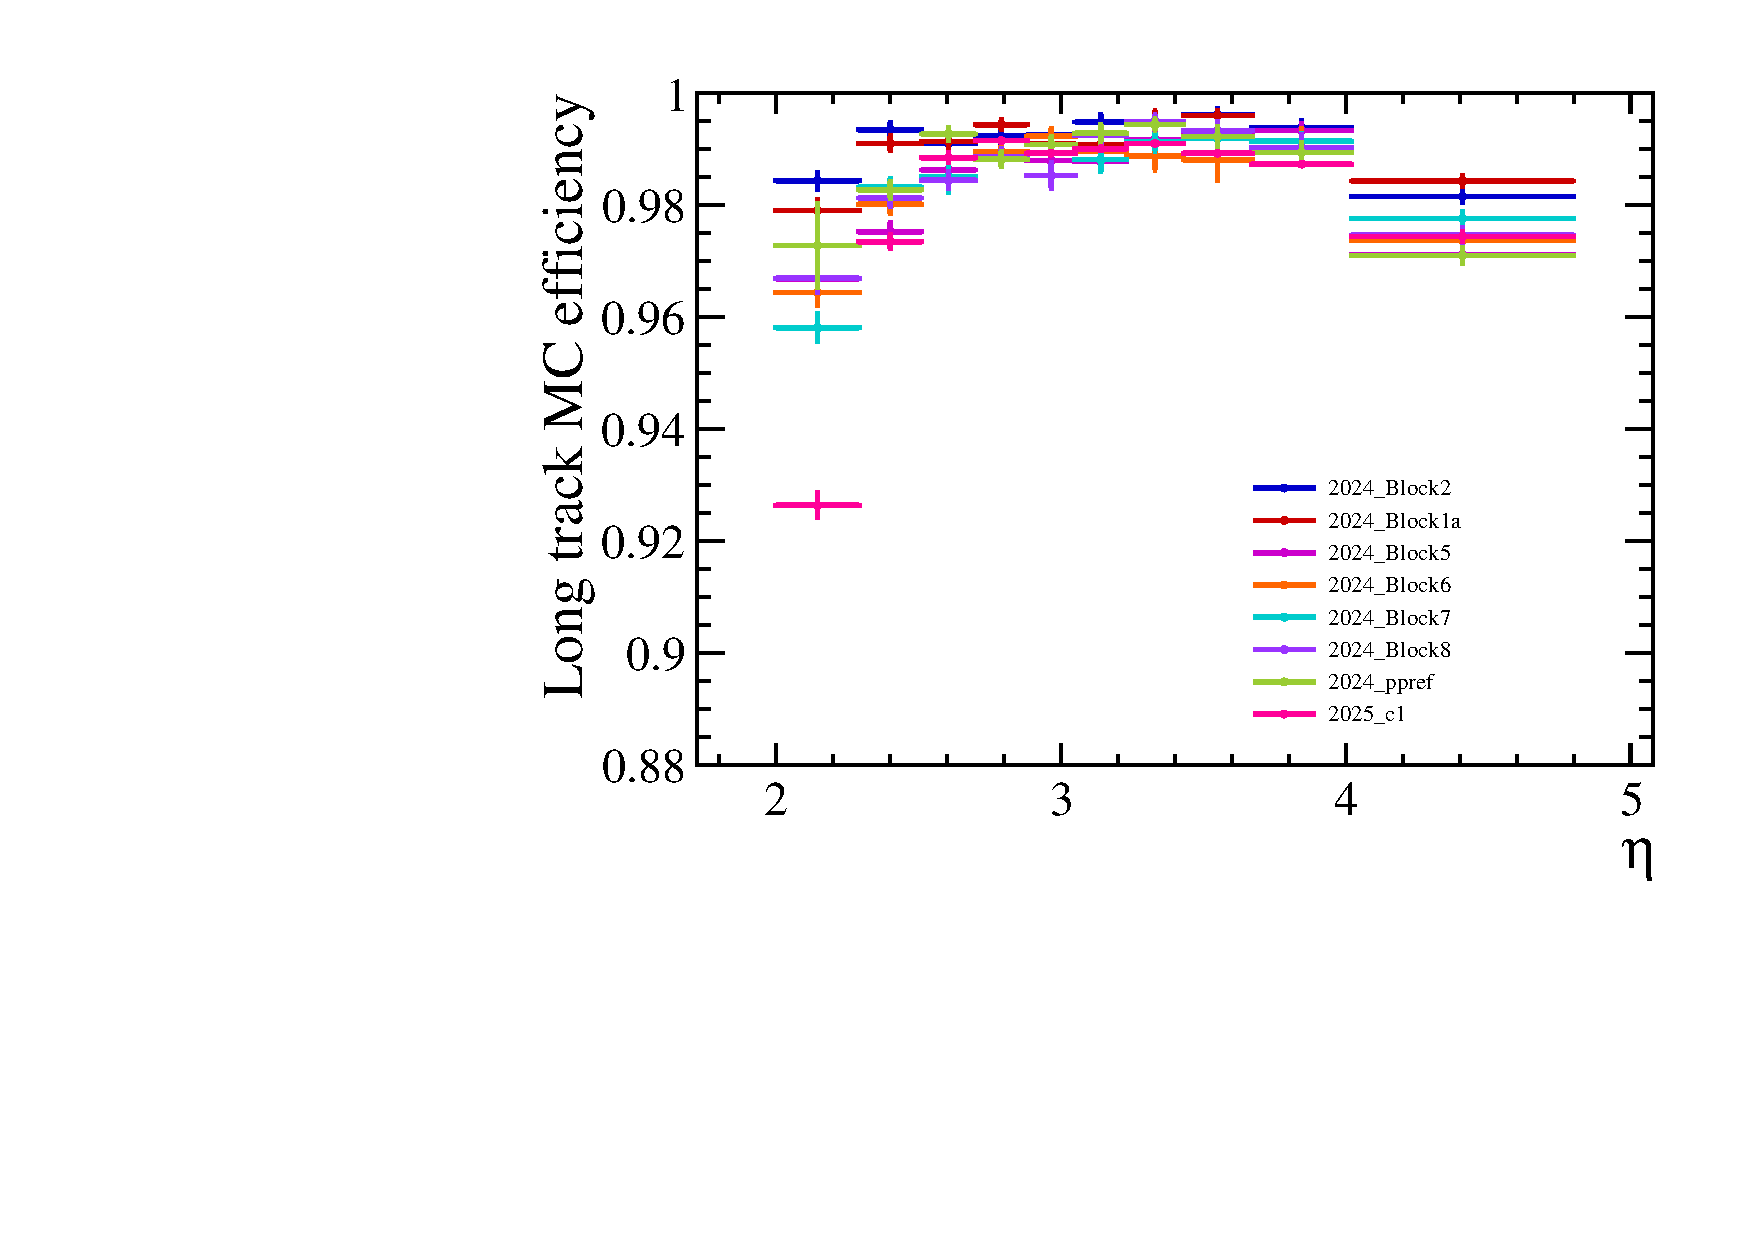
\includegraphics[width=0.75\textwidth]{Plots/trackeff_MC_MuonUT_ETA_respruced_samples.pdf}
    \end{subfigure}
  \end{figure}
\end{frame}

\begin{frame}{General observations}
  \vspace{0.0cm}
  {\large General observations on tracking efficiencies:}
  \vspace{0.2cm}
  \begin{enumerate}
    \setlength\itemsep{1.0em}
    \item{All data sets show consistent trends}
    \item{Performance seems to (slowly) drop over time}
  \end{enumerate}
  \vspace{0.4cm}
  {\large This is very encouraging! Several issues resolved, including:}
  \vspace{0.2cm}
  \begin{enumerate}
    \setlength\itemsep{1.0em}
    \item{Unusually high efficiencies in blocks 7/8}
    \item{Missing binds when rerunning reconstruction}
    \item{Large charge asymmetries in MuonUT samples}
  \end{enumerate}
  \vspace{0.2cm}
  {\large However, the low Velo efficiency in 2025 MC needs to be understood, so we will wait with the release of 2025 results}
\end{frame}

\begin{frame}{Tracking efficiency data/MC ratio}
  \vspace{0.0cm}
  {\large Data/MC ratio}
  \begin{figure}[htb]
    \centering
    \begin{subfigure}{0.5\textwidth}
      \centering
      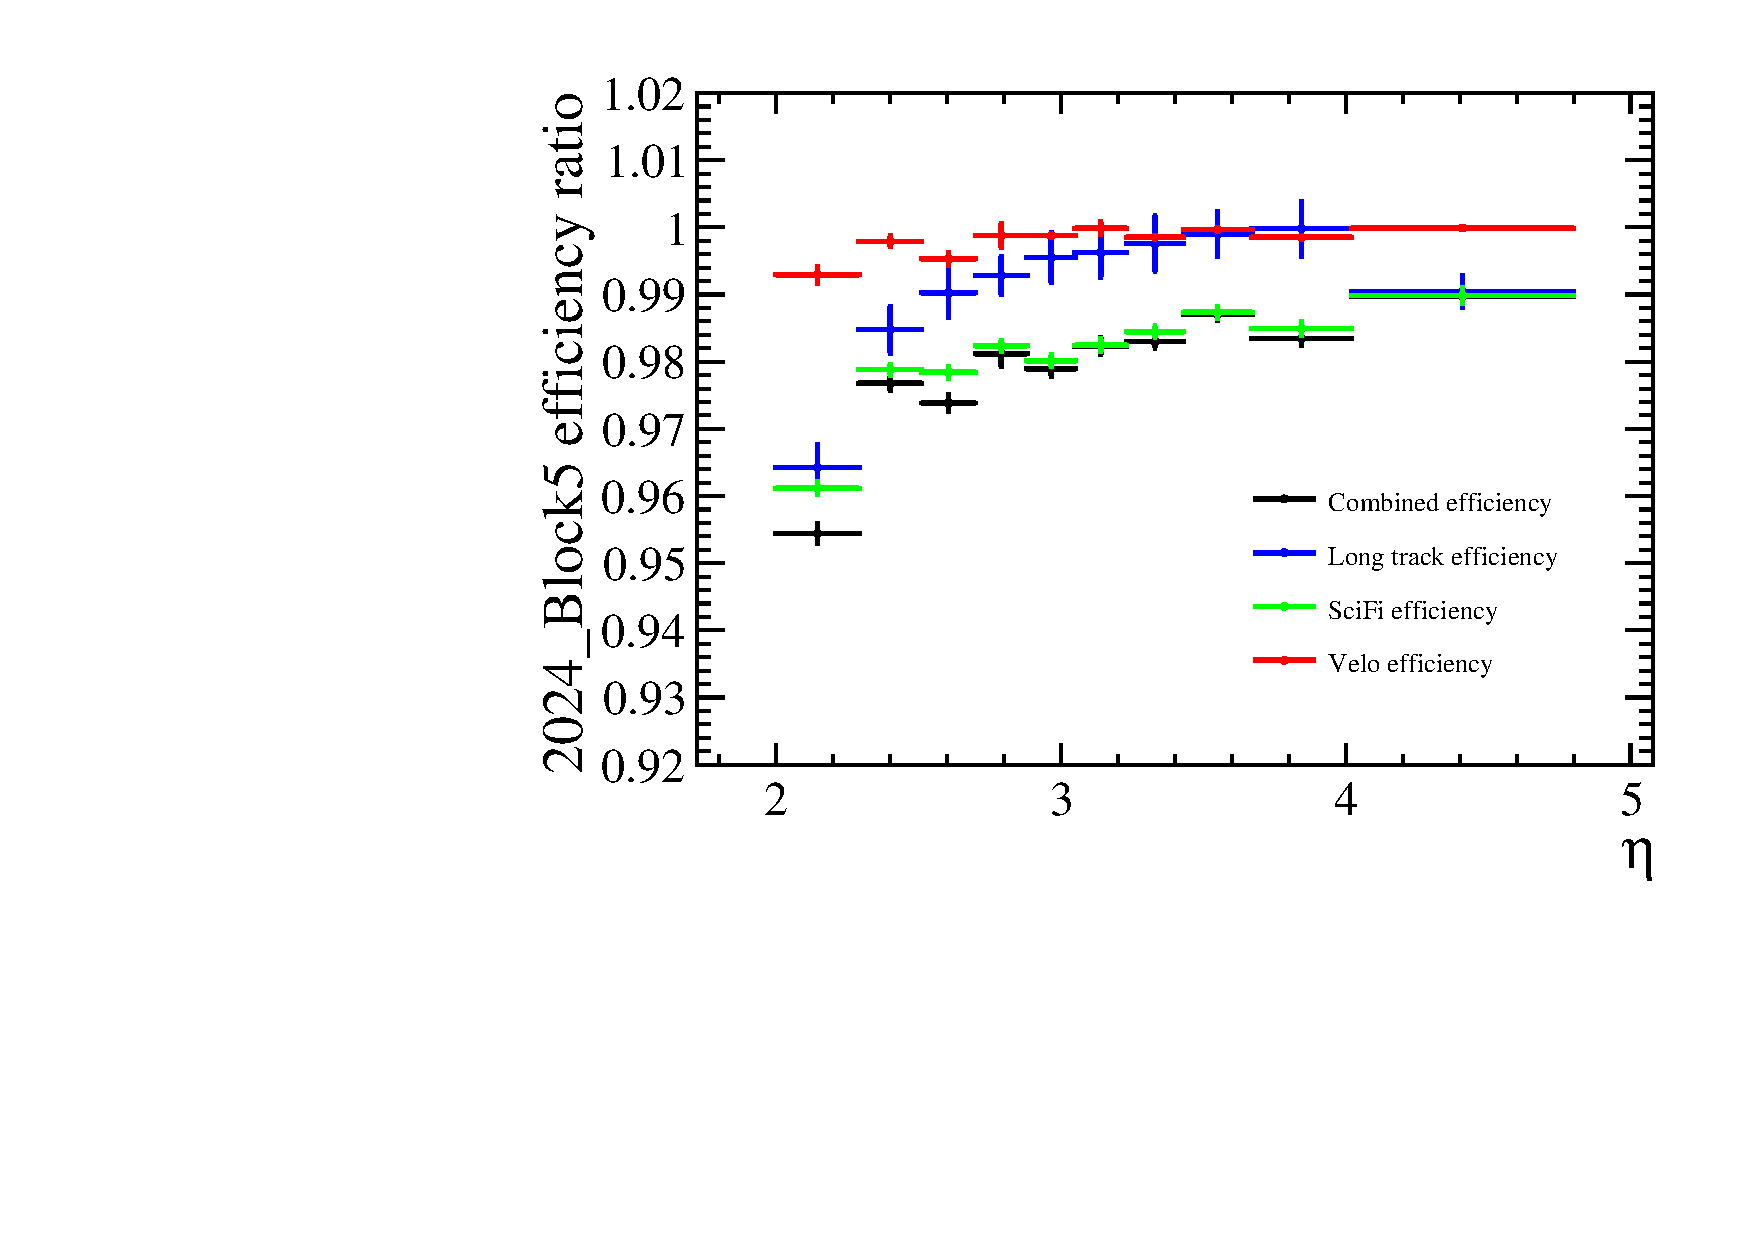
\includegraphics[width=1.0\textwidth]{Plots/trackeff_ratio_ETA_2024_Block5_respruced_samples.pdf}
    \end{subfigure}%
    \begin{subfigure}{0.5\textwidth}
      \centering
      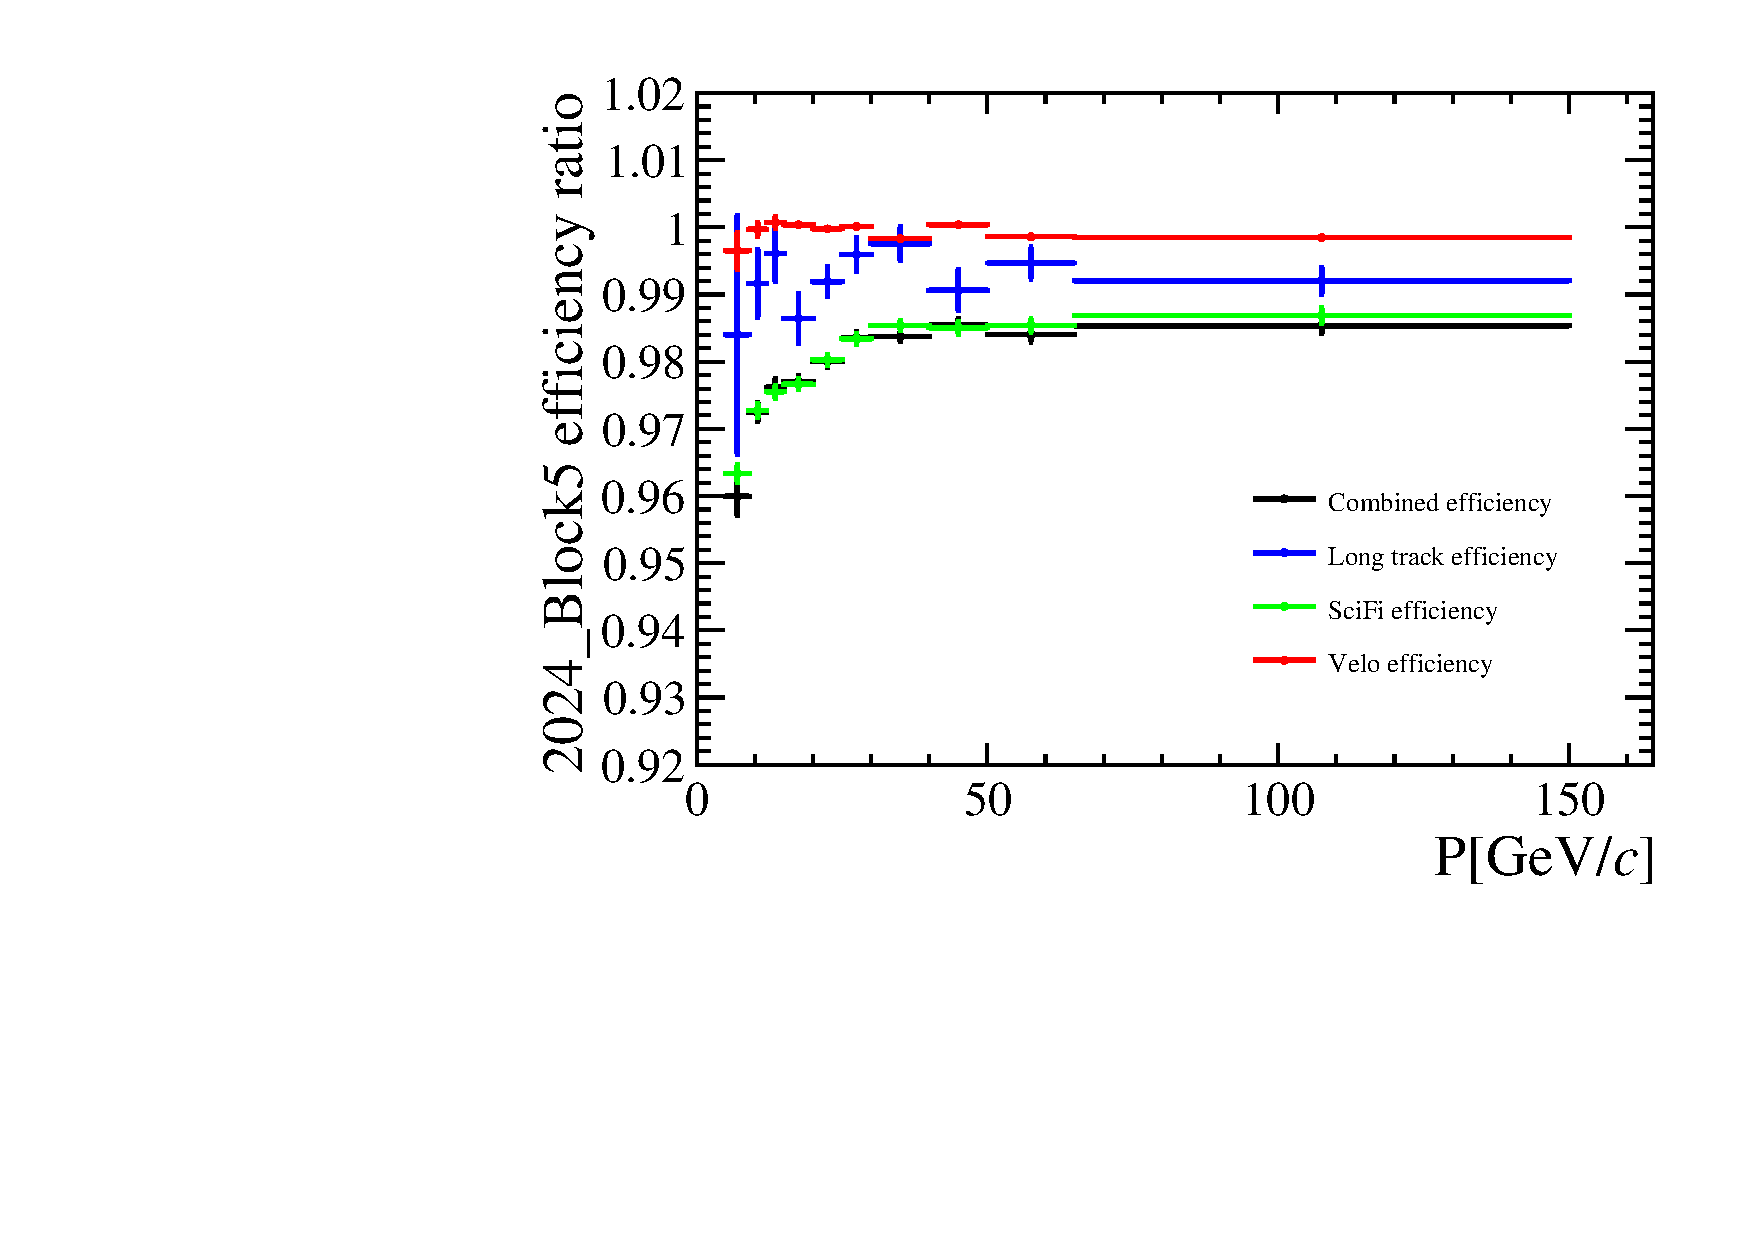
\includegraphics[width=1.0\textwidth]{Plots/trackeff_ratio_P_2024_Block5_respruced_samples.pdf}
    \end{subfigure}
  \end{figure}
  {Data/MC ratio for Combined/MuonUT track efficiencies block 5}
\end{frame}

\begin{frame}{Tracking efficiency data/MC ratio}
  \vspace{0.0cm}
  {\large Data/MC ratio}
  \begin{figure}[htb]
    \centering
    \begin{subfigure}{0.5\textwidth}
      \centering
      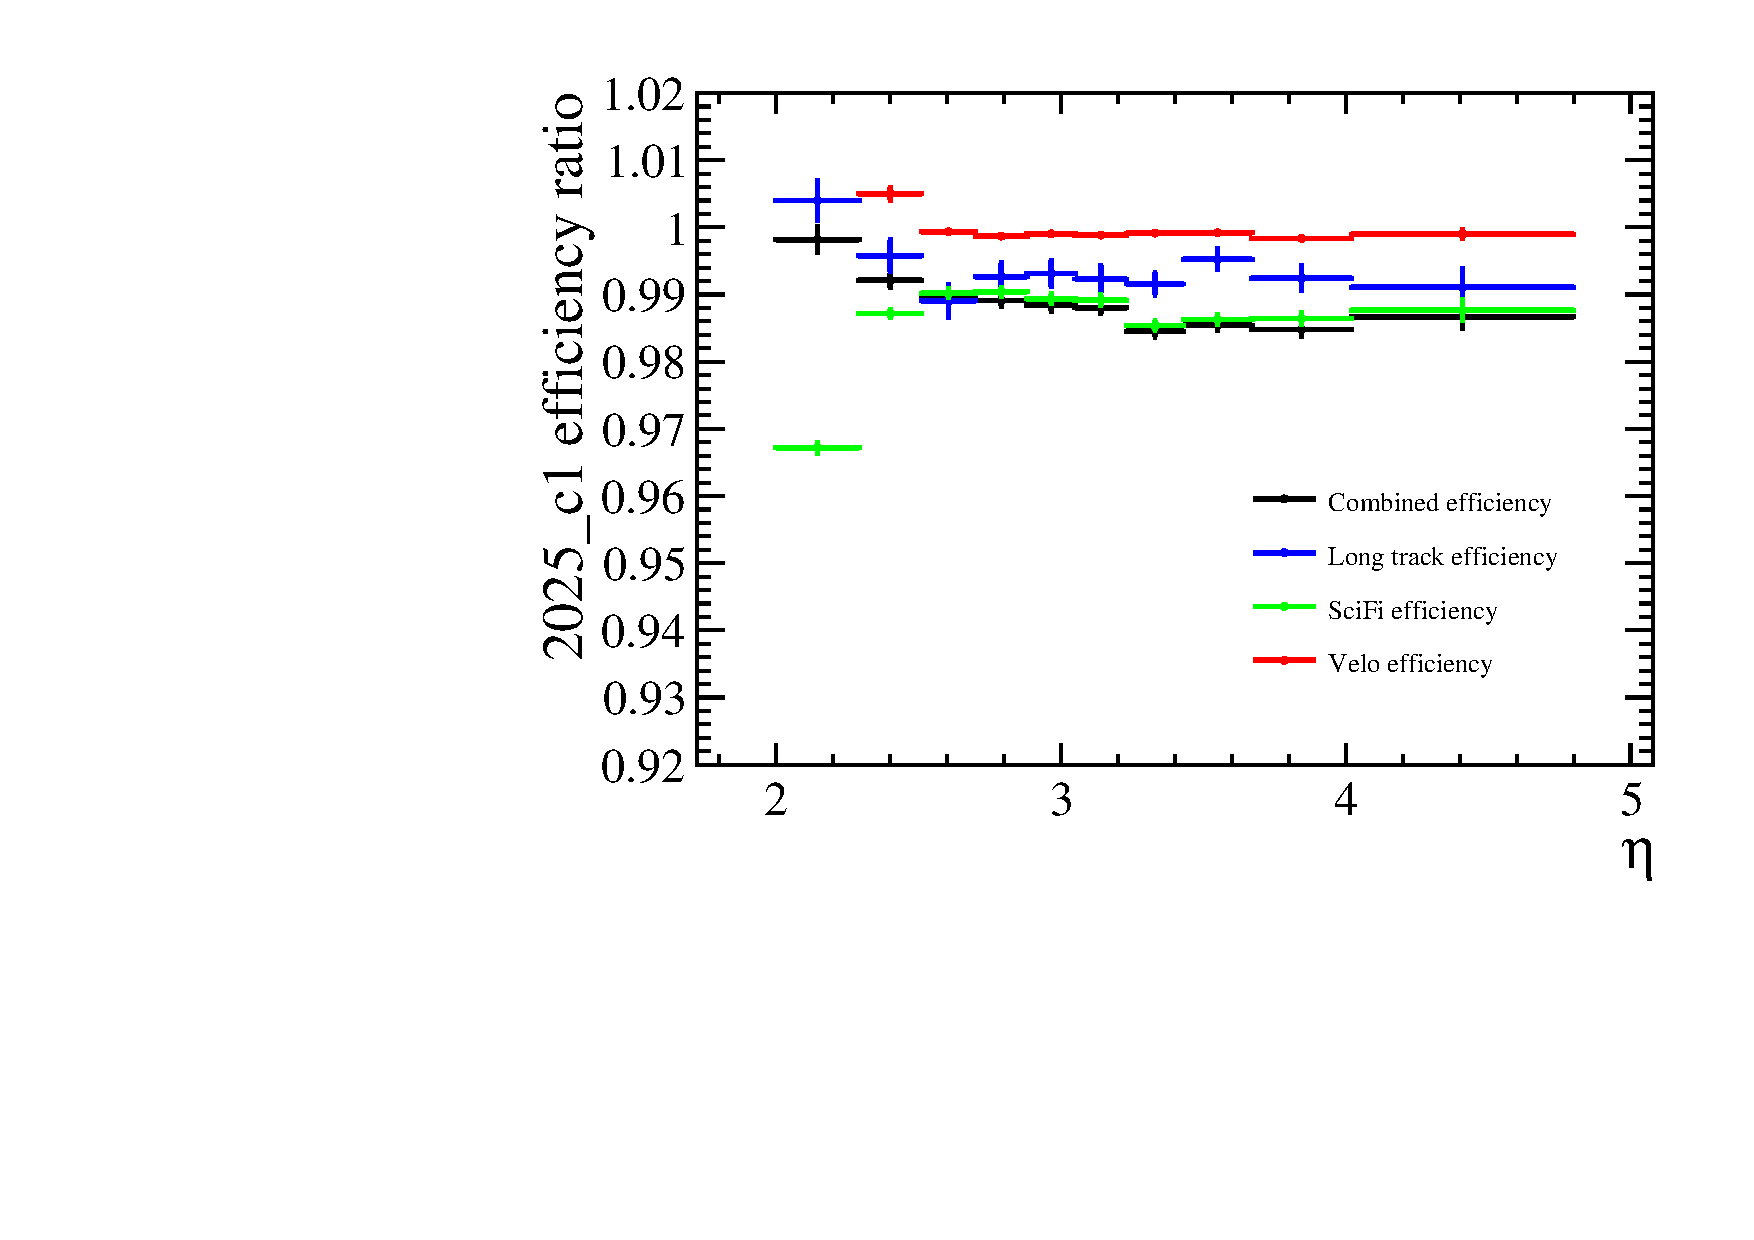
\includegraphics[width=1.0\textwidth]{Plots/trackeff_ratio_ETA_2025_c1_respruced_samples.pdf}
    \end{subfigure}%
    \begin{subfigure}{0.5\textwidth}
      \centering
      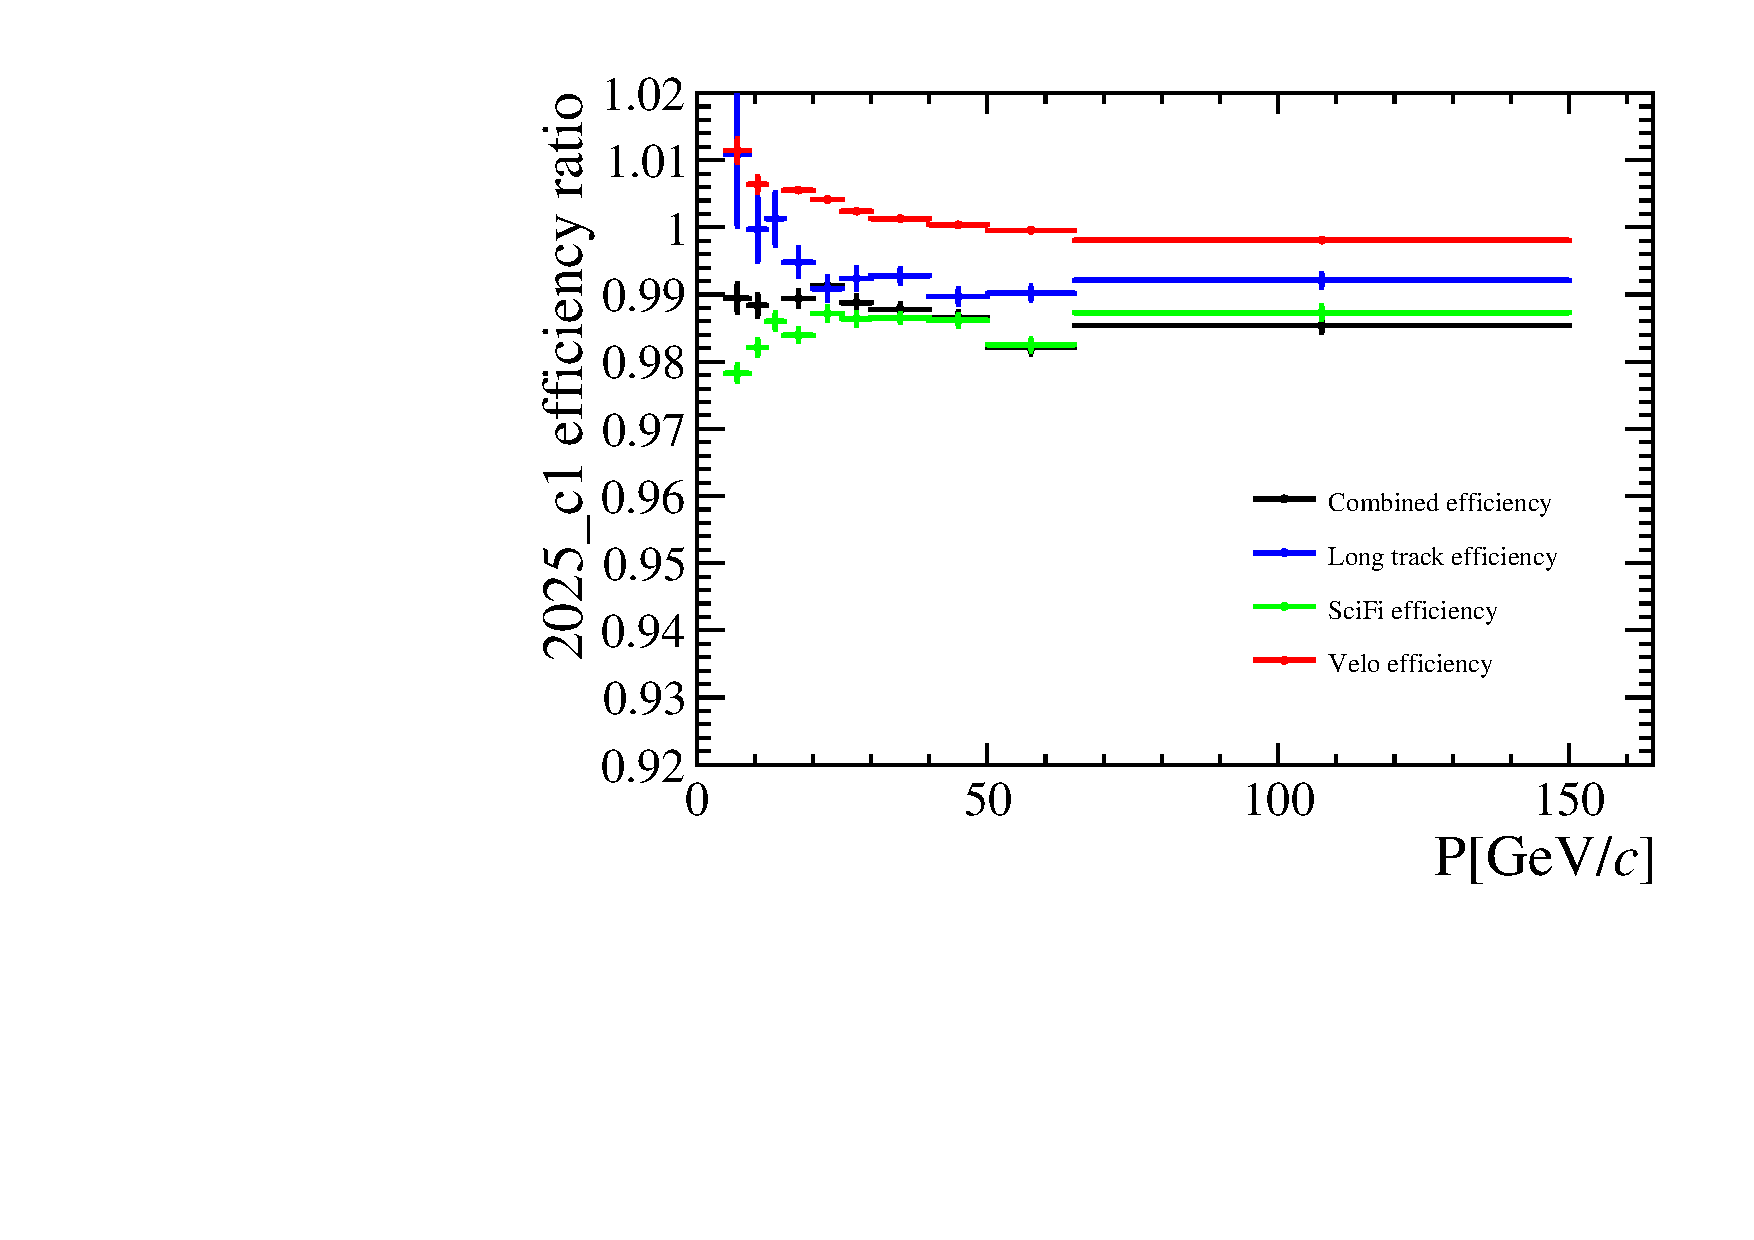
\includegraphics[width=1.0\textwidth]{Plots/trackeff_ratio_P_2025_c1_respruced_samples.pdf}
    \end{subfigure}
  \end{figure}
  {Data/MC ratio for Combined/MuonUT track efficiencies 2025 pre-TS}
\end{frame}

\begin{frame}{General observations}
  \vspace{0.0cm}
  {\large General observations on tracking efficiency ratios:}
  \vspace{0.2cm}
  \begin{enumerate}
    \setlength\itemsep{1.0em}
    \item{Velo efficiencies in 2024 are well described, but underestimated in MC for 2025}
    \item{Combined efficiency is mostly driven by SciFi efficiency}
    \item{Generally there is a $1$--$2\%$ discrepancy between Combined and MuonUT efficiencies, but effect is larger at low $p$ and low $\eta$, so discrepancies are smaller in 2D (next slide)}
    \item{Data--MC differ by almost $5\%$ at low $p$ and low $\eta$ and needs to be understood}
  \end{enumerate}
\end{frame}

\begin{frame}{Block 1a vs 1b}
  \vspace{0.0cm}
  {\large Do we need to split Block 1 into Block 1a and Block 1b?}
  \vspace{0.4cm}
  \begin{itemize}
    \setlength\itemsep{1.5em}
    \item{SciFi T2L0Q0M1H0 FE was excluded on 17th August}
    \item{Integrated luminosities are $0.92$~fb$^{-1}$ and $0.31$~fb$^{-1}$, respectively}
    \item{SciFi effectively has a hole in the 3rd quadrant}
  \end{itemize}
\end{frame}

\begin{frame}{Block 1a vs 1b}
  \vspace{0.0cm}
  {\large Block 1a (left) vs 1b (right)}
  \begin{figure}[htb]
    \centering
    \begin{subfigure}{0.5\textwidth}
      \centering
      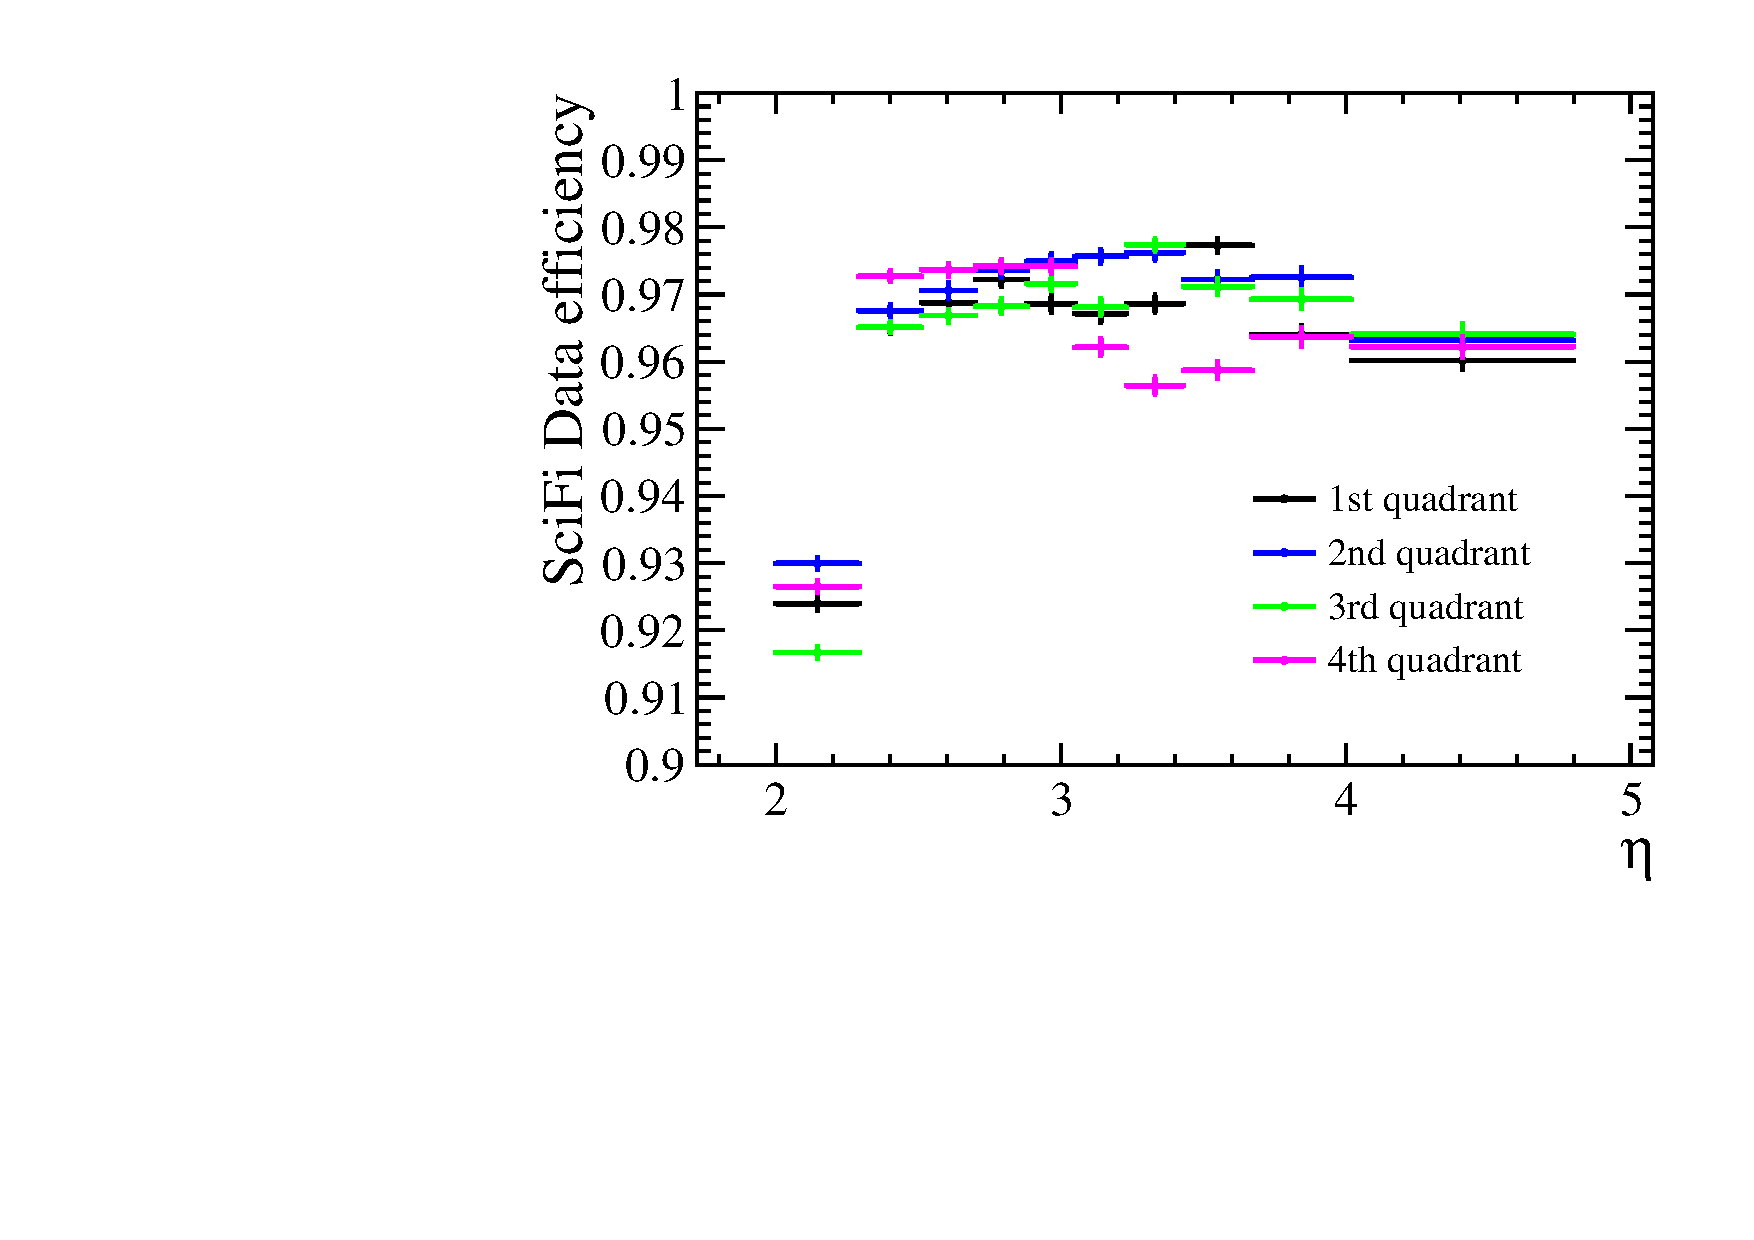
\includegraphics[width=0.75\textwidth]{Plots/trackeff_Data_VeloMuon_ETA_2024_Block1a_samples.pdf}
    \end{subfigure}%
    \begin{subfigure}{0.5\textwidth}
      \centering
      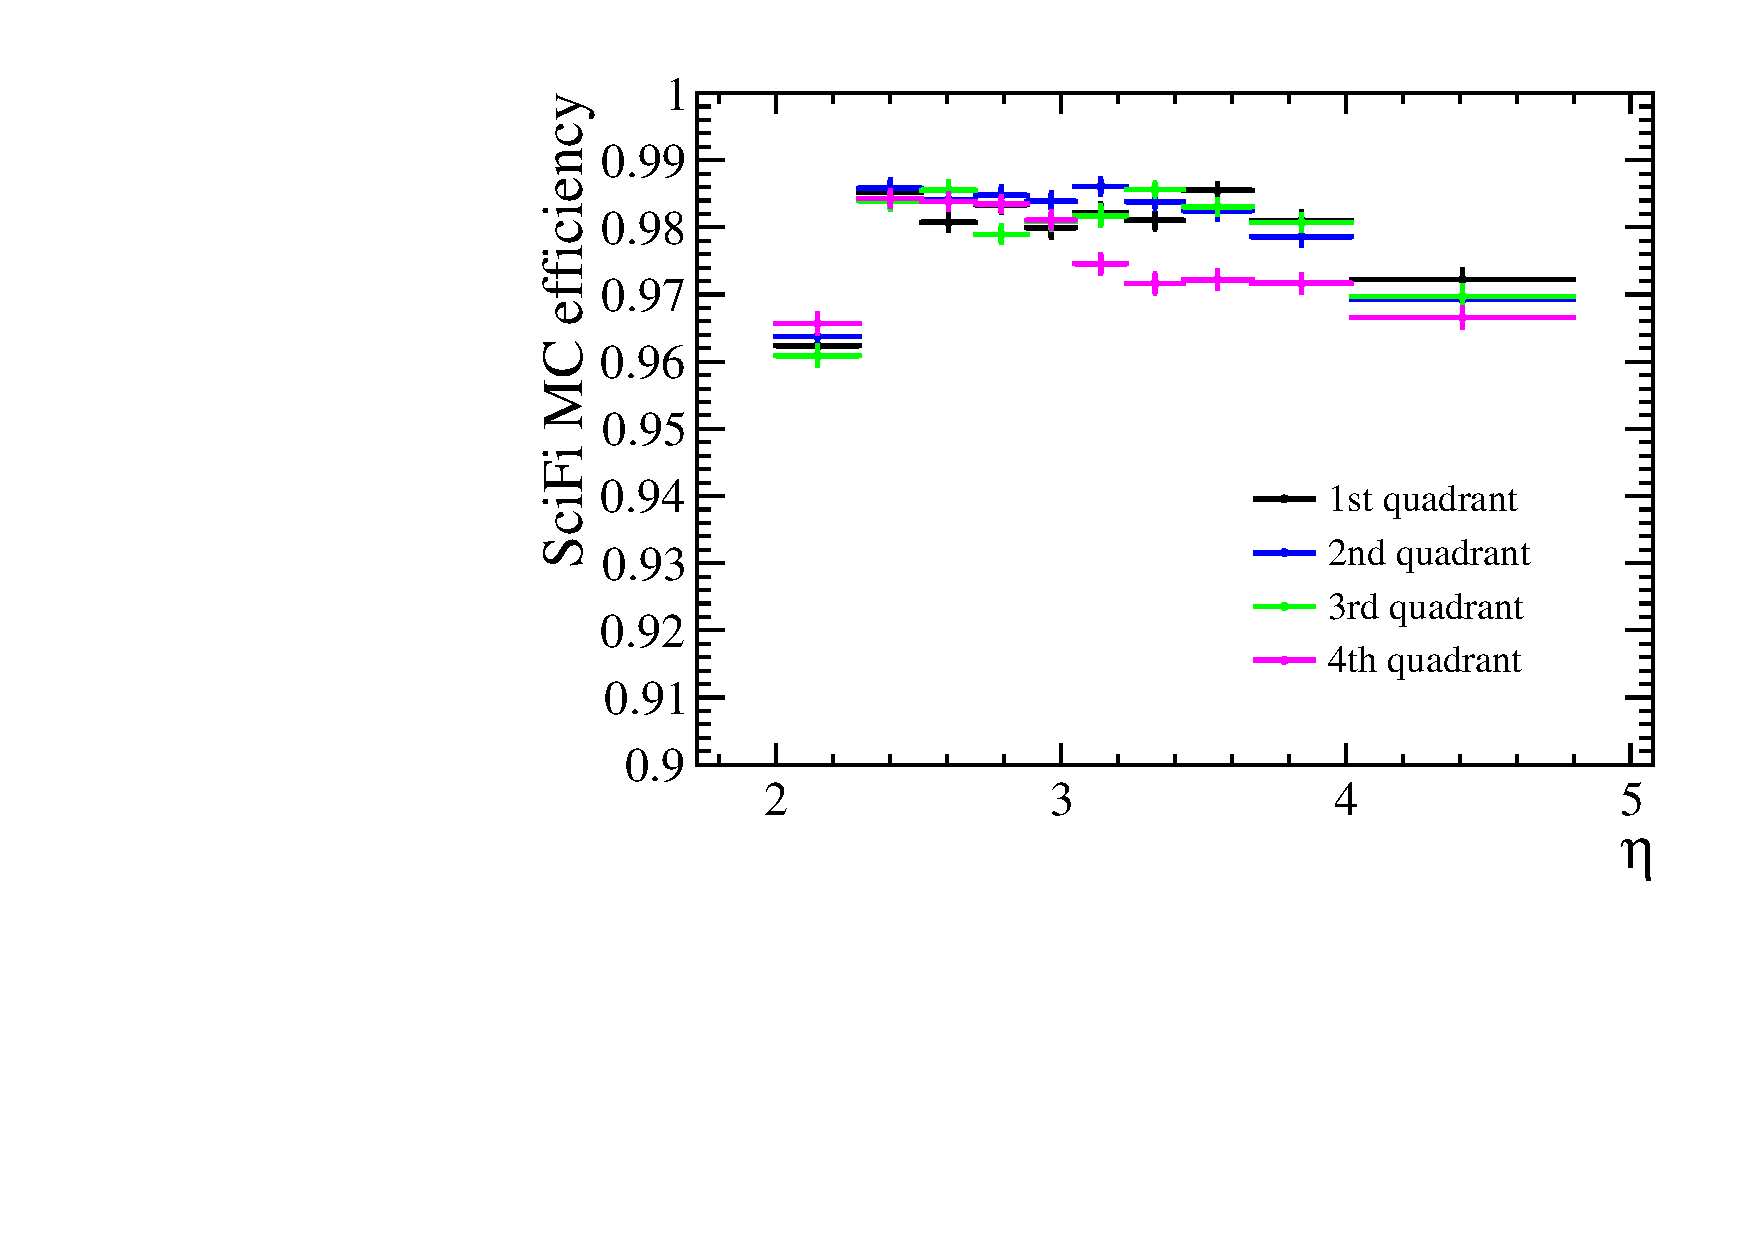
\includegraphics[width=0.75\textwidth]{Plots/trackeff_MC_VeloMuon_ETA_2024_Block1a_samples.pdf}
    \end{subfigure}
    \begin{subfigure}{0.5\textwidth}
      \centering
      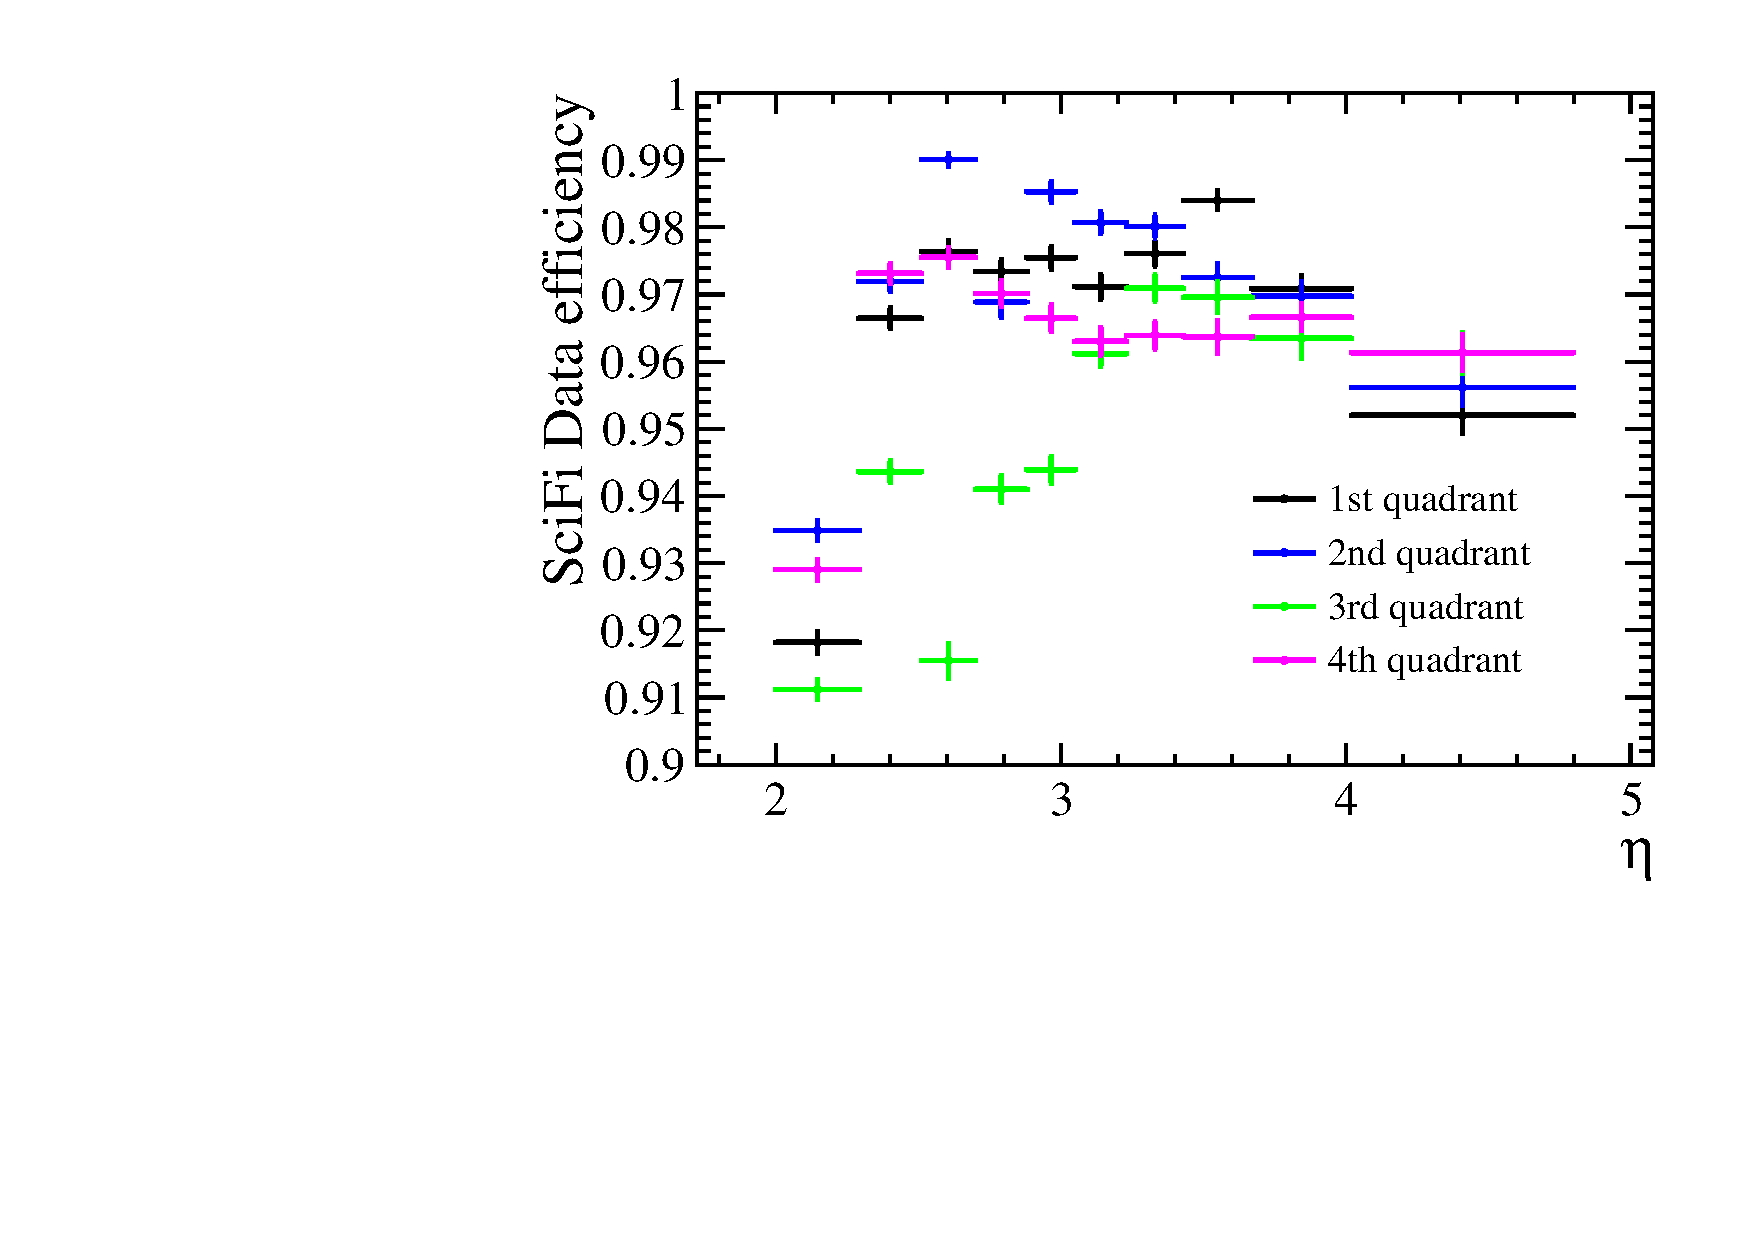
\includegraphics[width=0.75\textwidth]{Plots/trackeff_Data_VeloMuon_ETA_2024_Block1b_samples.pdf}
    \end{subfigure}%
    \begin{subfigure}{0.5\textwidth}
      \centering
      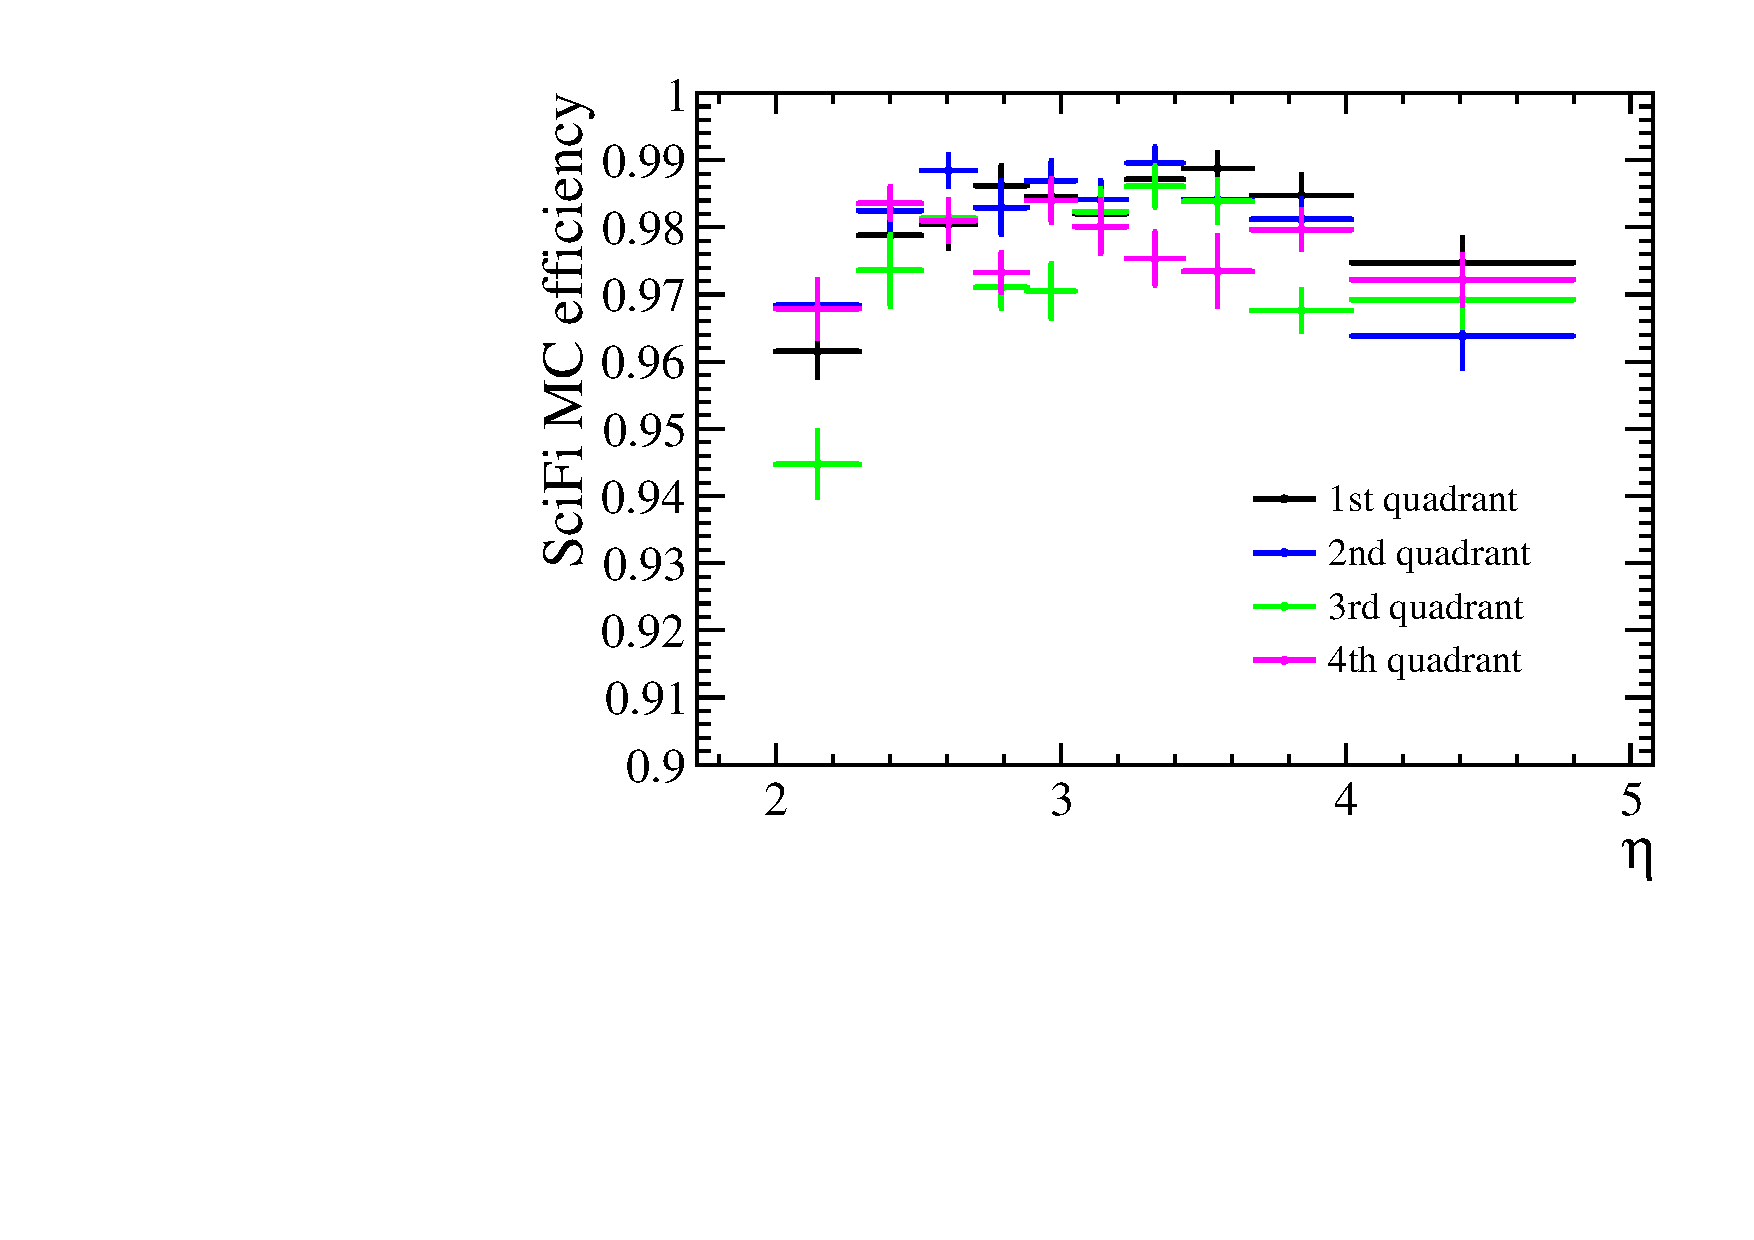
\includegraphics[width=0.75\textwidth]{Plots/trackeff_MC_VeloMuon_ETA_2024_Block1b_samples.pdf}
    \end{subfigure}
  \end{figure}
\end{frame}

\begin{frame}{Block 1a vs 1b}
  \vspace{0.0cm}
  {\large MC doesn't seem to describe the drop in tracking efficiency well...}
  \vspace{0.2cm}
  \begin{itemize}
    \setlength\itemsep{1.5em}
    \item{We will check with Simulation people}
    \item{Note: The ``hole'' in the SciFi is only visible when looking at tracks in the 3rd quadrant, the integrated numbers show negligible differences between block 1a and block 1b}
    \item{For now, tracking efficiencies are only provided for block 1a}
    \item{Analyses that are sensitive to this hole should exclude block 1b, other analyses can use results for block 1a as a proxy for block 1b}
  \end{itemize}
\end{frame}

\begin{frame}{2D binning}
  \vspace{0.0cm}
  \begin{itemize}
    \setlength\itemsep{1.0em}
    \item{Currently we have 1D bins in $p$ and $\eta$ with 10 bins each}
    \item{Using $10\times10$ 2D bins is impossible}
    \begin{itemize}
      \setlength\itemsep{0.3em}
      \item{Insufficient statistics at high (low) $p$ and low (high) $\eta$}
      \item{But most bins \underline{do} have sufficient statistics}
    \end{itemize}
    \item{Strategy: Start with $10\times10$ bins and merge bins}
    \begin{itemize}
      \setlength\itemsep{0.3em}
      \item{Only consider MC, which is important for constraining the fit shape}
      \item{Only consider VeloMuon yields, as Downstream efficiencies are close to $100\%$ anyway and MuonUT is only used as a cross check}
      \item{Try to merge bins along $\eta$ at high $p$ and vice versa}
      \item{Aim for roughly $\gtrsim 100$ matched candidates in each bin}
    \end{itemize}
    \item{The next plots contain many (tiny) numbers, apologies for this!}
  \end{itemize}
\end{frame}

\begin{frame}{2D binning}
  \vspace{0.0cm}
  {\large Final 2D binning in $p$ vs $\eta$ with 72 bins:}
  \vspace{-0.3cm}
  \begin{figure}[htb]
    \centering
    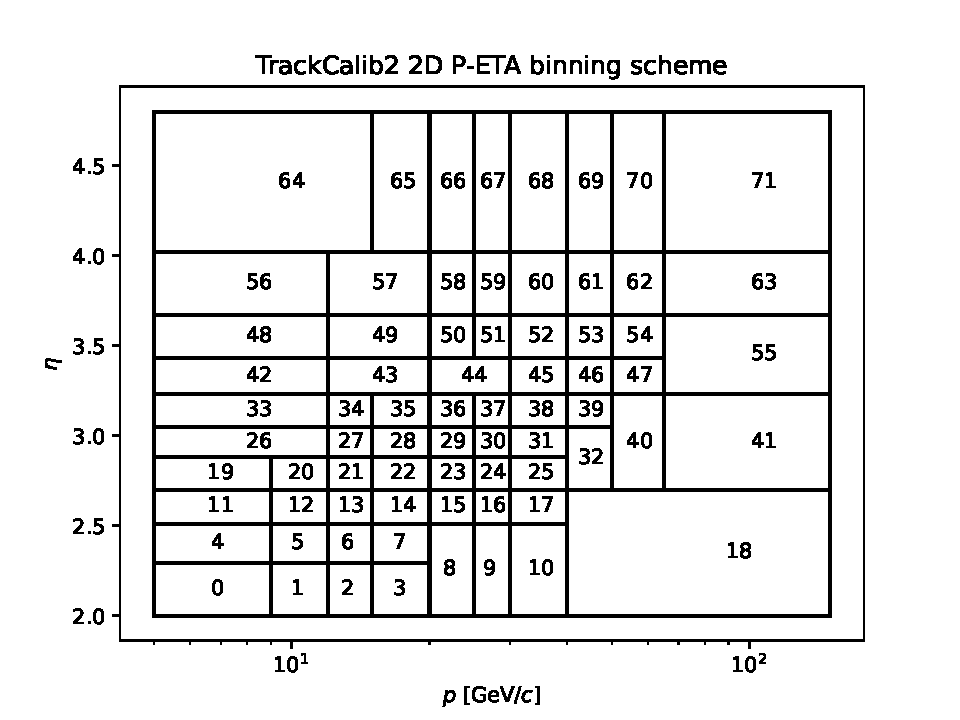
\includegraphics[width=0.8\textwidth]{Plots/TrackCalib2_2D_binning_scheme.pdf}
  \end{figure}
\end{frame}

\begin{frame}{2D binning}
  \vspace{0.0cm}
  \begin{figure}[htb]
    \centering
    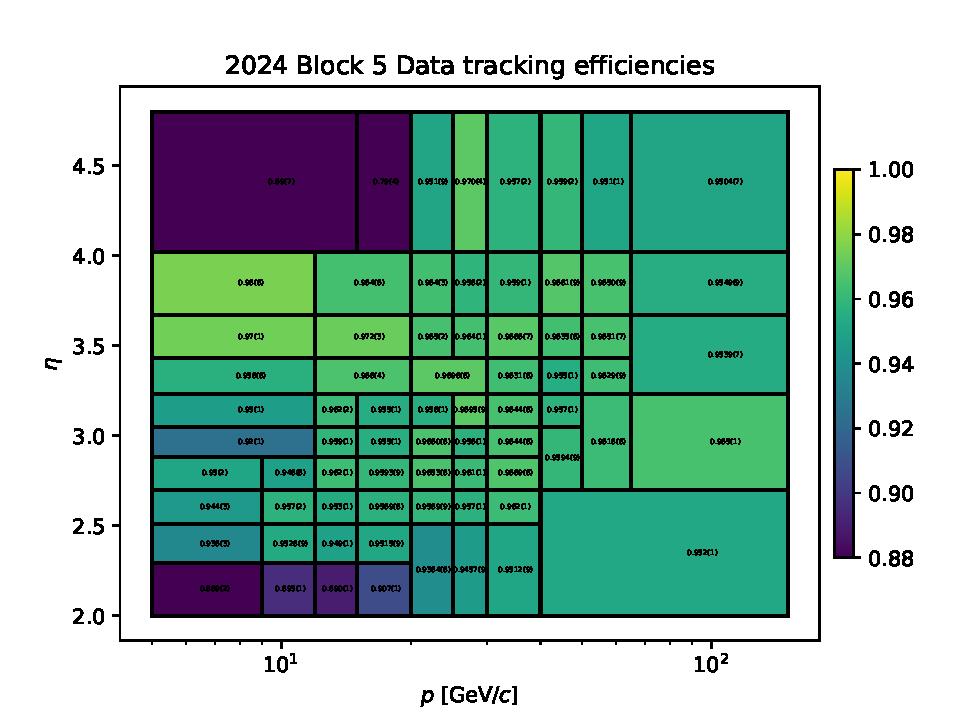
\includegraphics[width=0.85\textwidth]{Plots/TrackingEfficiencies_2D_binning_2024_Block5_Data_colour.pdf}
  \end{figure}
\end{frame}

\begin{frame}{2D binning}
  \vspace{0.0cm}
  \begin{figure}[htb]
    \centering
    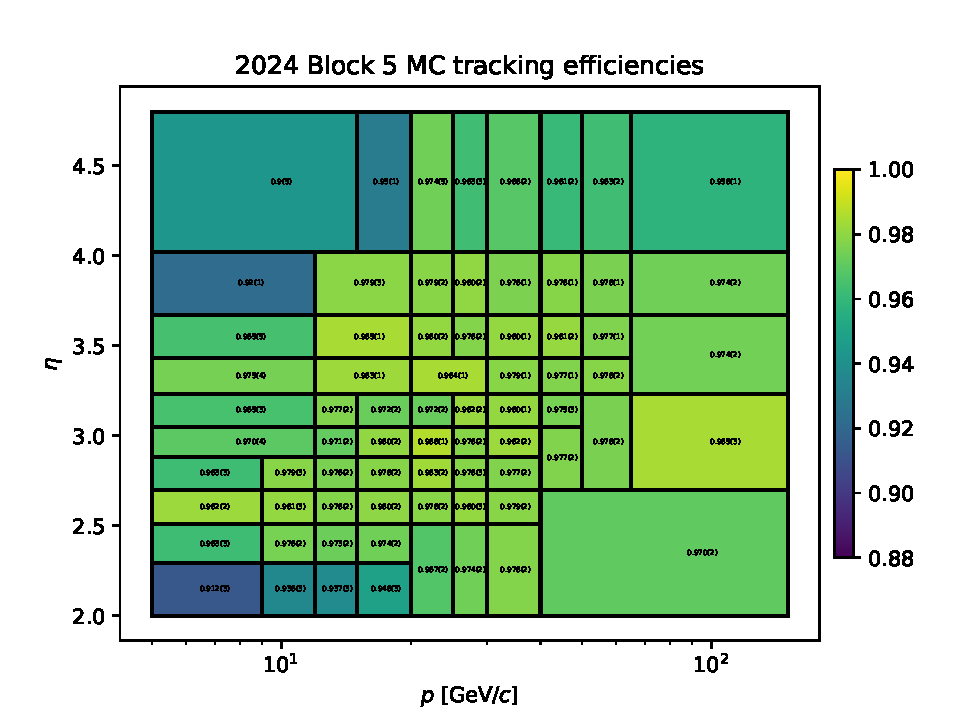
\includegraphics[width=0.85\textwidth]{Plots/TrackingEfficiencies_2D_binning_2024_Block5_MC_colour.pdf}
  \end{figure}
\end{frame}

\begin{frame}{2D binning}
  \vspace{0.0cm}
  \begin{figure}[htb]
    \centering
    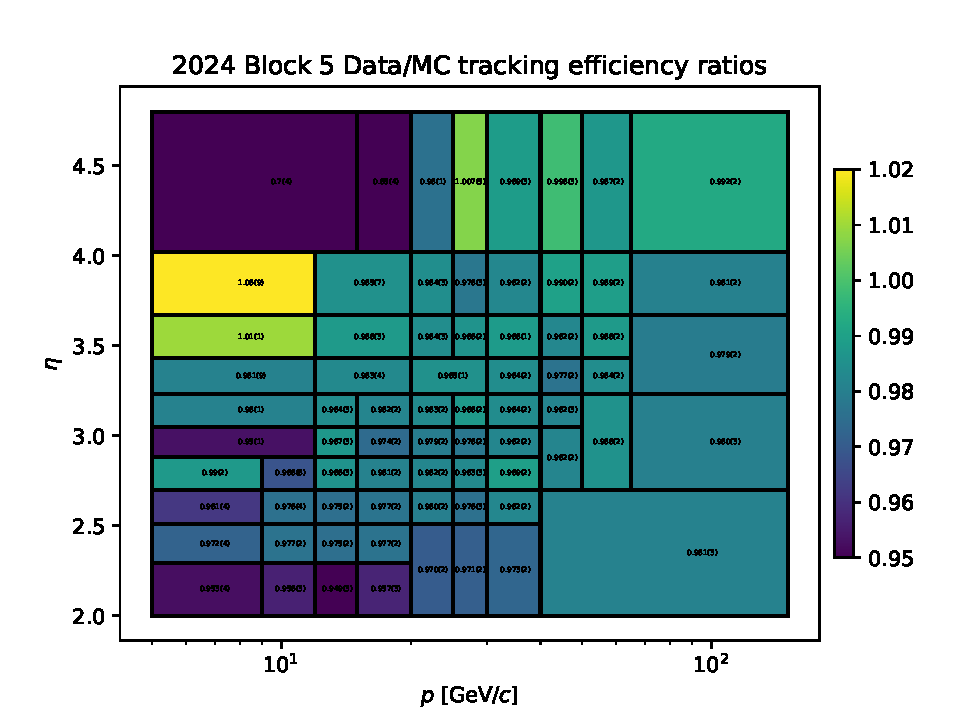
\includegraphics[width=0.85\textwidth]{Plots/TrackingEfficiencies_2D_binning_2024_Block5_Ratio_colour.pdf}
  \end{figure}
\end{frame}

\begin{frame}{2D binning}
  \vspace{0.0cm}
  \begin{figure}[htb]
    \centering
    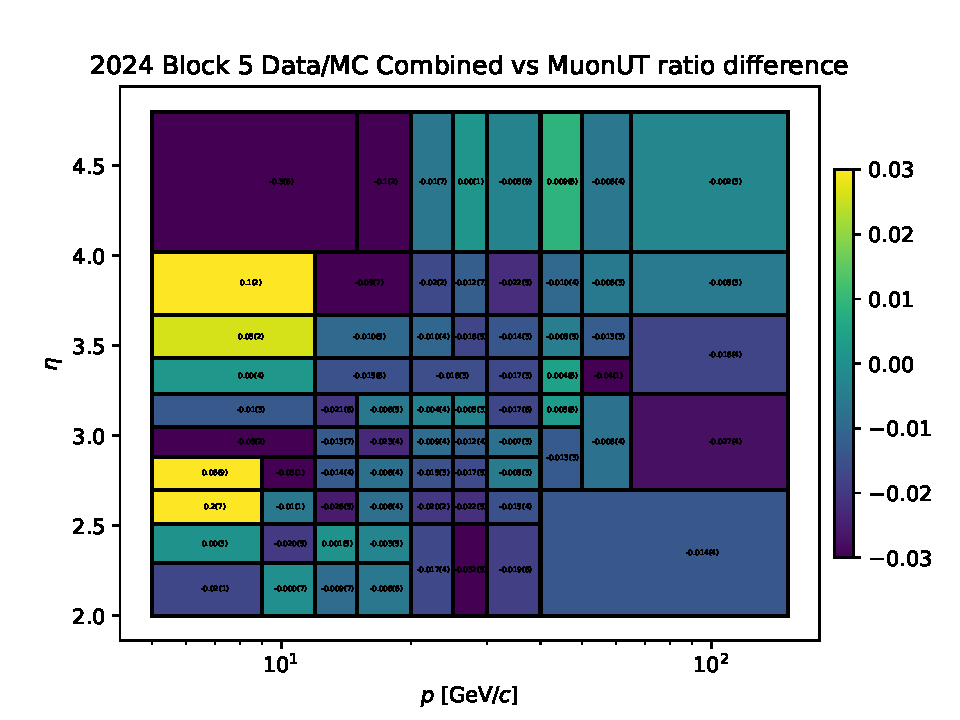
\includegraphics[width=0.85\textwidth]{Plots/TrackingEfficiencies_2D_binning_2024_Block5_RatioDiff_colour.pdf}
  \end{figure}
\end{frame}

\begin{frame}{2D binning}
  \vspace{0.5cm}
  {\large Note: After some feedback, the 2D binning will be slightly modified}
  \begin{itemize}
    \item{Merge bins 64 and 65}
    \item{Add a single high $p$ bin and a low $\eta$ bin}
    \item{These are bins with low statistics, but could be useful for some analyses to have}
  \end{itemize}
  \begin{figure}[htb]
    \centering
    \begin{subfigure}{0.5\textwidth}
      \centering
      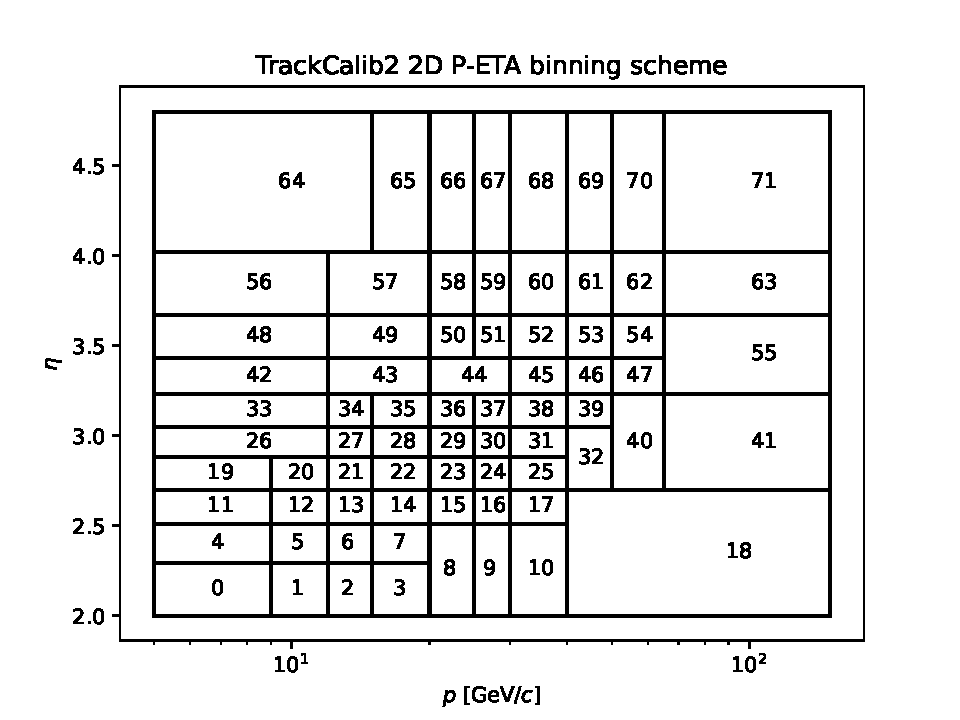
\includegraphics[width=1.0\textwidth]{Plots/TrackCalib2_2D_binning_scheme.pdf}
    \end{subfigure}%
    \begin{subfigure}{0.5\textwidth}
      \centering
      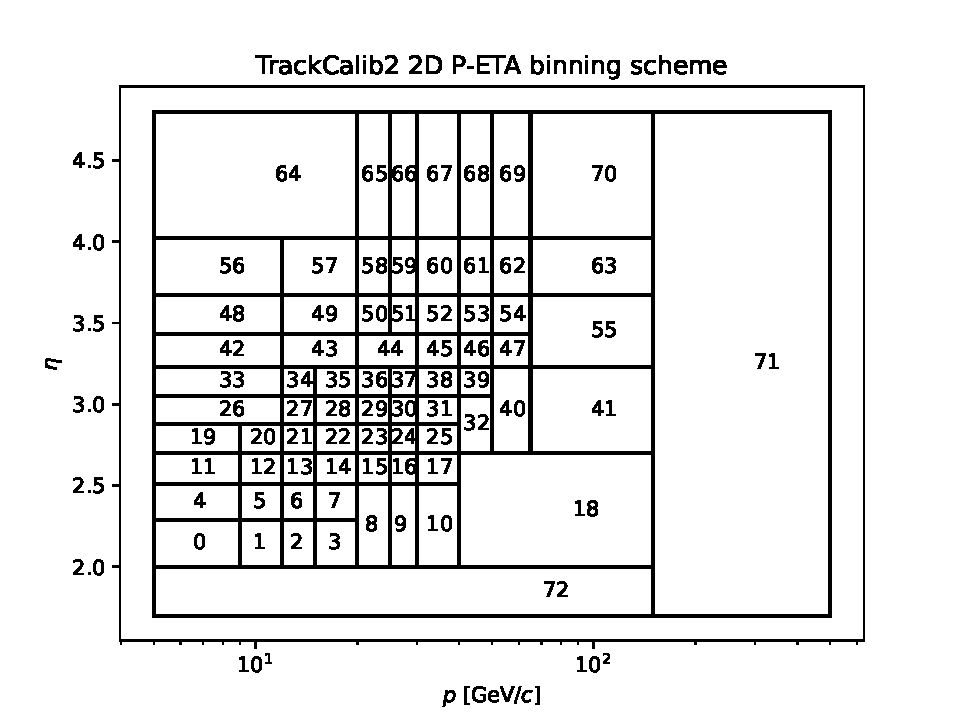
\includegraphics[width=1.0\textwidth]{Plots/TrackCalib2_2D_binning_scheme_new.pdf}
    \end{subfigure}
  \end{figure}
  \begin{figure}[htb]
    \centering

  \end{figure}
\end{frame}

\begin{frame}{Combined vs MuonUT systematic}
  \vspace{0.0cm}
  {\large Combined vs MuonUT systematic strategy?}
  \begin{itemize}
    \setlength\itemsep{1.0em}
    \item{Clearly depends on kinematics, so we should use 2D binning}
    \item{It's a method systematic, should not depend on dataset with same $\mu$}
    \item{Our current strategy:}
    \begin{enumerate}
      \setlength\itemsep{0.5em}
      \item{Determine ratio difference for all data sets in each bin}
      \item{Combine blocks 5/6 and 7/8}
      \item{Use blocks 5/6 as proxy for blocks 1/2 due to bug in MuonUT trigger line (see \href{https://gitlab.cern.ch/lhcb/Rec/-/merge_requests/4047}{!4047} and \href{https://gitlab.cern.ch/lhcb/Rec/-/merge_requests/4050}{!4050})}
      \item{For bins with a discrepancy above $1\,\sigma$, assign the difference from zero as a systematic}
      \item{Systematic will most likely be small in most bins, but a small number of bins might have a $1\%$--$2\%$ systematic, in rare cases $> 3\%$}
    \end{enumerate}
  \end{itemize}
\end{frame}

\begin{frame}{Release of tracking efficiencies}
  \vspace{0.0cm}
  {\large How should analysts use these results?}
  \vspace{0.2cm}
  \begin{itemize}
    \setlength\itemsep{1.0em}
    \item{Binning schemes are defined in JSON files}
    \item{Data/MC ratio in 2D bins provided for physics analysis, also as JSON}
    \item{Version 0 is available as a GitLab project \href{https://http.cat/status/102}{here}}
    \item{Version 1 will come soon}
    \begin{enumerate}
      \item{Waiting for large MC production to finish}
      \item{Separate $\mu^+$ and $\mu^-$ results as well}
      \item{Updated 2D binning scheme}
    \end{enumerate}
  \end{itemize}
\end{frame}

\begin{frame}{Hadronic corrections}
  \vspace{0.0cm}
  {\large {\color{red}Stuff from Fabian}}
  \begin{itemize}
    \setlength\itemsep{1.0em}
    \item{}
  \end{itemize}
\end{frame}

\begin{frame}{Summary and next steps}
  \vspace{0.0cm}
  \begin{itemize}
    \setlength\itemsep{1.0em}
    \item{Tracking efficiencies v0 for 2024 can now be used by analysts}
    \item{Issues to follow up on:}
    \begin{itemize}
      \item[-]{Block 1b MC}
      \item[-]{2025 Velo efficiencies}
    \end{itemize}
    \item{Waiting for large MC production before next release}
    \item{{\color{red}Hadronic corrections due to uncertainty in material budget shows promising results, and corrections will be made available very soon}}
  \end{itemize}
  \vspace{0.2cm}
  \begin{center}
    \Huge Thanks for your attention!
  \end{center}
\end{frame}

\end{document}
